% !TeX spellcheck = en_US
\documentclass[journal]{IEEEtran}
\usepackage[utf8]{inputenc}
\usepackage{graphicx}      % include this line if your document contains figures
%\usepackage{natbib}        % required for bibliography
\usepackage{todo}
\usepackage{amsmath}
\usepackage{amsfonts}
\usepackage{amsbsy}
\usepackage{printlen}
\usepackage{acronym}
\usepackage{mathtools}
\usepackage{enumitem}
\usepackage{tabularx}
%\usepackage{caption}
\usepackage[caption=false]{subfig}
%\usepackage{hyperref}
\usepackage{tikz}
\usepackage[europeanresistors,americaninductors]{circuitikz}
%\usepackage{comment}
%===============================================================================
\renewcommand{\todo}{\Todo}
\newcommand{\vect}[1]{\boldsymbol{#1}}
\newcommand{\tr}{^\intercal}
\newcolumntype{Y}{>{\centering\arraybackslash}X}
\newcommand\T{\rule{0pt}{2.6ex}}       % Top strut
\newcommand\B{\rule[-1.2ex]{0pt}{0pt}} % Bottom strut
%\usepackage{color}
%\definecolor{darkgreen}{rgb}{0,0.75,0}
%\hypersetup{
%	pdfauthor={Geir Hovland, Pål Johan From, Lars Imsland, Jostein Bakkeheim, Morten Hovd}, %
%	pdftitle={Sample article for Modeling, Identification and Control based on pdfLaTeX},
%	pdfkeywords={MIC,pdflatex,vector graphics},
%	pdfsubject={MIC Journal Article},
%	colorlinks=true,
%	citecolor=darkgreen,
%	urlcolor=darkgreen,
%	pdfstartview=Fit,
%	pdfpagelayout=SinglePage,
%	pdfcreator=pdflatex,
%	pdfproducer=pdflatex}
\newcommand{\url}[1]{#1}


\begin{document}
 \acrodef{MPC}{model predictive control}
 \acrodef{FDI}{fault detection and identification}
 \acrodef{FTC}{fault-tolerant control}
 \acrodef{ESD}{Energy Storage Device}
 \acrodef{DP}{Dynamic Positioning}

\title{Marine Vessel and Power Plant System Simulator\footnote{The authors of this paper are funded by the project Design to verification of control systems for safe and energy efficient vessels with hybrid power plants (D2V), where the Research Council of Norway is the main sponsor. NFR: 210670/070}} 
% Title, preferably not more than 10 words.

%TODO check membership
\author{Torstein I. Bø,~\IEEEmembership{Member,~IEEE,}
	Andreas R. Dahl,~\IEEEmembership{Member,~IEEE,}
	Tor A. Johansen,~\IEEEmembership{Member,~IEEE,}
	Eirik~Mathiesen,~\IEEEmembership{Member,~IEEE,}
	Michel R. Miyazaki,~\IEEEmembership{Member,~IEEE,}
	Eilif Pedersen,~\IEEEmembership{Member,~IEEE,}
	Roger~Skjetne,~\IEEEmembership{Member,~IEEE,}
	Asgeir J. Sørensen,~\IEEEmembership{Member,~IEEE,}
	Laxminarayan Thorat,~\IEEEmembership{Member,~IEEE,}
	Kevin~K.~Yum,~\IEEEmembership{Member,~IEEE}
\thanks{T.I. Bø and T.A. Johansen are with Center for Autonomous Marine Operations and Systems, Department of Engineering Cybernetics, Norwegian University of Science and Technology, 7491
	Trondheim, Norway (e-mail: torstein.bo@itk.ntnu.no)}
\thanks{E. Mathiesen is with Kongsberg Maritime AS}%
\thanks{A.R. Dahl, Michel R. Miyazaki, Eilif Pedersen, Roger Skjetne, Asgeir Sørensen, Ingrid Utne and Kevin K. Yum are with Center for Autonomous Marine Operations and Systems, Department of Marine Technology, Norwegian University of Science and Technology}%
}%



% The paper headers
\markboth{IEEE Journal of Oceanic Engineering}%
{Bø \MakeLowercase{\textit{et al.}}: System Simulator of Marine Vessel and Power Plant}
\maketitle

  \begin{abstract}
A modern marine vessel with electric propulsion has many systems.
These systems need to interact with each other and cannot be studied independently.
This is especially important when considering fault scenarios, harsh weather, and complex integrated operations.
Often simulation of a vessel with dynamic positioning (DP) and diesel-electric propulsion is done with two separate simulators; one for the vessel motion with the DP controller and one for the diesel-electric power plant.
This paper presents a system simulator where these two simulators are combined.
The main contribution of this paper is the presentation of the required models for the integration.
Most of the models are based on well known model, while some new are developed to fit the need of the simulator.
These new models are verified against models of higher fidelity.

The marine power system simulator is developed to serve as platform to provide high degree of accuracy in modeling and simulation of typical configurations of complex electrical power system on board a marine vessel. 

The simulator is developed using MATLAB/Simulink with top-to-bottom overview of marine power and propulsion system to mimic single line diagram.
The component models for diesel engines, generators, thrusters, propellers, and other subsystems are mostly based on well known models from the literature.
A case study is included, where a DP ship and a drilling vessel is used for some typical operations and fault scenarios.
\end{abstract}

\begin{IEEEkeywords}
	Marine technology, Marine vehicles, Power system simulation
\end{IEEEkeywords}



\subsection{Introduction}
\subsubsection{Shipboard electrical system}
The on-board electric power system is crucial for most modern marine operations, especially for vessels that use electricity for propulsion. Diesel-electric propulsion is common in offshore vessels with dynamic positioning (DP).

The ability to counteract positioning disturbances such as current, waves and wind depends on the power plant capacity. 
Insufficient power may result in decreased DP performance and loss of position. 
More severely, a total loss of electric power, known as a blackout, results in loss of control of the vessel.

Redundancy in power capacity, distribution and in the number of generating units is one possible alleviation of the risk of power system faults.
This is the standard for DP operations that require high-reliability, such as drilling or diving.

Redundancy, however, is costly. Economical expenses are significant, both in terms of investment in equipment which most of the time is not strictly necessary, and in terms of machine running hours which lead to more frequent maintenance. Also, in an environmental perspective, running generators at loads significantly lower than the designed optimum entails increased emissions and fuel consumption.

The mentioned concerns motive the development of new power plant control strategies and the introduction of new power sources. Such steps are not trivial, due to the complex and strongly interconnected nature of on-board marine power plants: the grid is weak, i.e. sensitive to changes both in produced and consumed power. Simulation is a valuable tool for investigating such effects at all stages of development and operation. 

This paper is an extension of~\cite{Bo2015}. However, more details of the models are included in this paper. In additions, verification of the new models and new cases in the case study are added.

\subsubsection{Previous work}
A great number of marine power plant simulation solutions exist. The intended use ranges from commercial to academic, and the content from a few state equations to complete software suites.

A selection of simulators follows:
\begin{description}
\item[Marine Cybernetics' CyberSea] technology platform encompasses models of hydrodynamics, electro-mechanics
and sensors \cite{MarineCybernetics2014}. It is used for hardware-in-the-loop
(HIL) testing~\cite{Johansen2009} and dynamic capability analysis (DynCap)~\cite{Pivano2014}.

%In addition to the dynamic positioning (DP) controller, the simulator includes \cite[Sec. 3.4]{JohansenFossenVik2005}:
%gensets, main consumers, PMS (including \cite{SmogeliTrondBoerhaugPivano2013}
%black-out prevention, load limitation and sharing, and auto-start
%and auto-stop of generators), thruster system interaction and failure
%modes. Beyond this, the level of modeling detail is not known.

\item[U.S. Office of Naval Research's] Electric Ship Research and Development Consortium studies include both real-time HIL simulators \cite{RenSteurerWoodruff2005}, models of higher fidelity \cite{SteurerAndrusLangstonQiSuryanarayananWoodruffRibeiro2007} and extension to hybrid plants \cite{xie2009analysis}.

\item[Marine Systems Simulator (MSS)] \cite{MSS2010} library and simulator for MATLAB/Simulink is a 2004 merge of \cite[Sec. 1]{MSS}: marine GNC toolbox \cite{Fossen2002},
MCSim \cite{SorensenPedersenSmogeli2003} and DCMV \cite{PerezBlanke2003}.
It includes vessel dynamics, environmental (wave, surface current,
and wind) forces and advanced thrust loss models.

\item[DNV GL's Sesame Marine] \cite{DNV2014} risk management software includes Marintek's
Simulation of Marine Operations (SIMO) motion and station keeping
simulator. The system is capable of modeling multibody systems and
flexible systems. %The documentation \cite{DNV2002} does not mention
%power systems explicitly. The thruster force is controlled by the
%DP controller, not specified to consider dynamic power limitations.

\item[Italian Integrated Power Plant Ship Simulator] includes an integrated
power system model implemented in the Simulink environment \cite{BosichFilippoGiulivoSulligoiTessarolo2012}. Real-time capabilities are not known.

\item[NTNU models]
include thruster power consumption \cite{Hansen2001} and PMS functions \cite{Radan2008}.

\item[NTNU bond graph]
model library \cite{Pedersen2012} includes a vessel model. The library is also verified through full-scale experiments.
\end{description}

Some solutions mainly focus on the electrical system without concern for the actual DP performance and related consumption, while others do the opposite.


\subsubsection{Design of System Simulators}
The simulator in this paper is a system simulator.
This means that the purpose of the simulator is to model interactions between each of the subsystems of the complete system.
Such a simulator should be flexible, such that many different cases can be studied.
This can be achieved by a modular design, where different models of a component can be chosen.

The use cases of the simulator will determine the dynamics which are necessary to model.
The difference in magnitude of the smallest and the largest timescale of the dynamics in such a multi-physics simulator may be in order of decades.
It is therefore important to decide the timescales which are important for the use cases.

The smallest timescale of the vessel can be found in the electric system and are in order of milliseconds, while the largest may be effects of wear and tear with order of months and years.
For simulator of short-circuit, the fast dynamics must be modeled; however, the effects of the environment, and wear and tear can be assumed to be constant.
On the other hand, the electric system can be assumed to be in steady state when simulating DP operation, as the timescales of the electric system is much faster than the timescale of the vessel motion.
Model reduction is necessary when models includes small timescales to keep the computational speed of the simulator at a reasonable level.
It is also important to keep the simulator consistent.
This means that when choosing a fidelity level with a given range of timescales, all effects of interest must be modeled.

The complexity of a system simulator grows with the number of components and the fidelity level.
By increasing the fidelity level, more parameters and a more throughly verification and validation is required.
For studies where high fidelity level is required it is seldom necessary for all the models to be of high fidelity.
We can therefore use high fidelity models on some of the models and low on others.
By using a modular design, it is easy to use low fidelity models to identify where higher fidelity is required.
These models can then be replaced with new high fidelity models.

One of the challenges with a system simulator is the validation of the simulator.
Due to the inherent high complexity, it may be difficult to validate the simulator.
Each of the submodels can be validated by themselves, but this does not validate the entire simulator, as important components can have been neglected and interaction effects can be important.
Other implementations of the system simulator can be used for validation, as long as they are already validated.
A small scale or full scale test can also be used for validation.
However, this is costly and time consuming.

\subsubsection{Use cases}\label{sec:use-cases}
The simulator has already been used in several studies considering DP with diesel-electric propulsion and additional consumers such as hotel loads and motors for drilling, compressors and pumps.

A selection of typical use cases follows:

\begin{description}

\item[Realistic power consumption profile:]Since the DP controller and thruster models are interconnected with the power plant, the power load fluctuates are represented in a realistic way. 
The interaction between the many control subsystems, such as PMS, thrust allocation, thruster torque or speed control, is included~\cite{Bo2013}.
The simulator can therefore be used to generate time series for later use in isolated subsystem simulation (e.g., diesel engine simulation). 

\item[Fault consequence analysis:]
The plant behavior in the event of an electrical fault, such as the loss of a genset, can be simulated~\cite{Bo2013b}. The resulting DP performance is then also available. This may improve the conventional capability analysis, which is calculated assuming the propulsion system is in steady-state. Indeed, transients during plant reconfiguration can be critical~\cite{Pivano2014}.

\item[Operation optimization:]
The detailed level of modeling includes many states for each submodule, for instance temperature and power output. Based on these, operation may be optimized with regards to emissions, maintenance or fuel consumption.

\item[Concept evaluation:]
Submodules representing new subsystems such as energy storage devices (ESD) can be interfaced to the simulator. For instance, this allows investigation of new power sources and their effect on the overall control and performance of the plant.

%\item[High fidelity thruster model] The simulator includes a thruster model that can be used as an %extension to the MSS toolbox~\cite{MSS}.
%During simulation of DP~operations it is normal to ignore the dynamics of the thrusters (or use very %simplified models) and to assume that the thrusters are able to generate the desired thrust command %given by the DP~controller.
%However, this assumption may be too rough in some cases, especially after a fault in the electric %propulsion system, as power constraints may be active.
%By including the presented extensions more realistic thruster dynamics can be simulated.
%The thruster model is based on the work in~\cite{Smogeli2006}.
%\item[Thruster induced load fluctuations]
%A known problem for vessels in DP~operation is large fluctuations of the power consumption by the %thrusters, due to wave-induced  variations of the advance velocity of the propeller. 
%This gives excessive wear and tear of the generator sets and frequency variations, and it should be %avoided by better control of the propeller~\cite{Sorensen2009,Veksler2014}.
%\item[Energy storage devices control]
%Recent development in the \ac{ESD} technology allowed the usage of those components to save fuel %and increase safety. Studies shows that the potential for fuel saving is high depending on the operation %\cite{Lindtjorn2014}. An integrated simulator allows the controller validation and potential fuel saving %estimation for each vessel operational profile. It is also possible to verify the vessel \ac{DP} system %influence due to the presence of an \ac{ESD}.
%Finally, the overall safety of the system can be analyzed, studying the resulting electrical system %robustness.

\end{description} 

It must be stressed that the simulator is not limited to diesel-electric propulsion, nor DP operations.

%The article continues with an overview of the simulator.
%Further, details of the models and simulator are described in the following sections.
%The article ends with a case study illustrating some capabilities of the simulator, before %further work and the conclusion.

\subsubsection{Contribution}
This paper proposes an integrated simulator of the electric power system together with the vessel motion including the DP system. 
All models required for this integration is included,, where most of the models are based on well known models.
However, some new models are established to achieve the desired fidelity level and performance of the simulator.
These models are verified with existing models.
The scope runs from high-level control systems, such as the positioning system and power management system (PMS), down to high-fidelity models of power generators, storage and consumers, such as gensets, batteries and thrusters, respectively.
The accuracy of the simulator is only verified qualitatively due to the complexity of the system.
Quantitatively verification of the plant is research still to be done and is considered outside the scope of this article.

The simulator is implemented as an extension to the MSS, adding the electrical power plant, machinery, and thrusters. The solution is module-based, allowing reconfiguration and tailoring of the plant with regards to subsystem modeling resolution. A single-line diagram representation is used in the electrical power module. The code is based on Simulink and is suitable for real-time simulation.

\section{Modeling}

\subsection{Simulator Overview}
Since the simulator is modular, many different designs and operations can be simulated.
The main focus has been to simulate vessels with diesel electric propulsion, e.g., ferries and cruise vessels in transit, or advanced drilling rigs in DP~operation, where the thruster control is constrained by the power available.
Vessels with hybrid propulsion may also be simulated.
Different operational modes may be simulated, as long as the desired thruster settings are available, either set manually or by a controller. 
Some operations may be transit operation, maneuvering, and DP~operation.

The main assumptions of the simulator are:
\begin{description}
\item[Steady-state electric system ] It is assumed that the electrical system is in steady state. This gives real-time capabilities, but some features can not be simulated.
The simulator captures dynamics with time scale down to 1 second.
However, the dynamics of the electric system are often around milliseconds and can therefore be assumed to be in steady state.
This is verified in Section~\ref{sec:elverification}.
The simulated electrical variables are frequency, voltage, active power, and reactive power.
It is therefore possible to simulate faults, such as under/over-frequency, slowly developing under/over voltage fault, and reverse power.
However, it is not able to simulate phase imbalance, transient voltage faults, short circuit, and harmonic distortion.
\item[Mean-value engine model] The diesel engines are modeled by mean-value engine models. This means that most of the components in the diesel engine system are mathematically modeled based on the physical laws. 
However, the in-cylinder process is simplified so that it gives only a cycle average output such as average shaft torque and mass and energy flow of the combustion gas.
\item[Power management system] The objective of the PMS is to make sure that there is always enough generator capacity for the electrical system. 
Additional generators could be started if too little power is available.
Loads may be commanded to reduce power or be disconnected to reduce the power consumption if required.
The PMS needs to know the status of the complete plant.
It is therefore connected to all producers and main consumers, in addition to the main switchboards and breakers.
\item[Protection relays] Protection relays are not modeled, as breakers can be tripped by a timer.
This means that some custom protection relays need to be implemented to simulate a partial blackout.
Alternatively, post-processing can be used to detect when breakers should be opened.
\item[Fixed pitch, variable speed thrusters] The thrusters are assumed to be fixed pitch propellers, with the possibility to run with variable speed.
Thrusters that can rotate in any direction, azimuth thrusters, and fixed direction thrusters (e.g., tunnel thrusters) can be simulated.
\end{description}

An object-oriented modeling structure has been used to model the marine power plant.
This means that each block in the simulator represents a physical component in the vessel, and further subsystem blocks represent internal physical components of the larger system.
The components are standalone and can be used in other simulators using Simulink or exported using Simulink Coder.

The top level view of the model is illustrated by an example in Fig.~\ref{fig:DPscheme}.
This view represents the information flow regarding motion control of the vessel.
A DP~controller has been used in the presented case.
Alternatively, the setpoints of the thrusters can be given manually during transit, maneuvering or other operations without DP~control.
\begin{figure*}[t!]
\normalsize
\centering
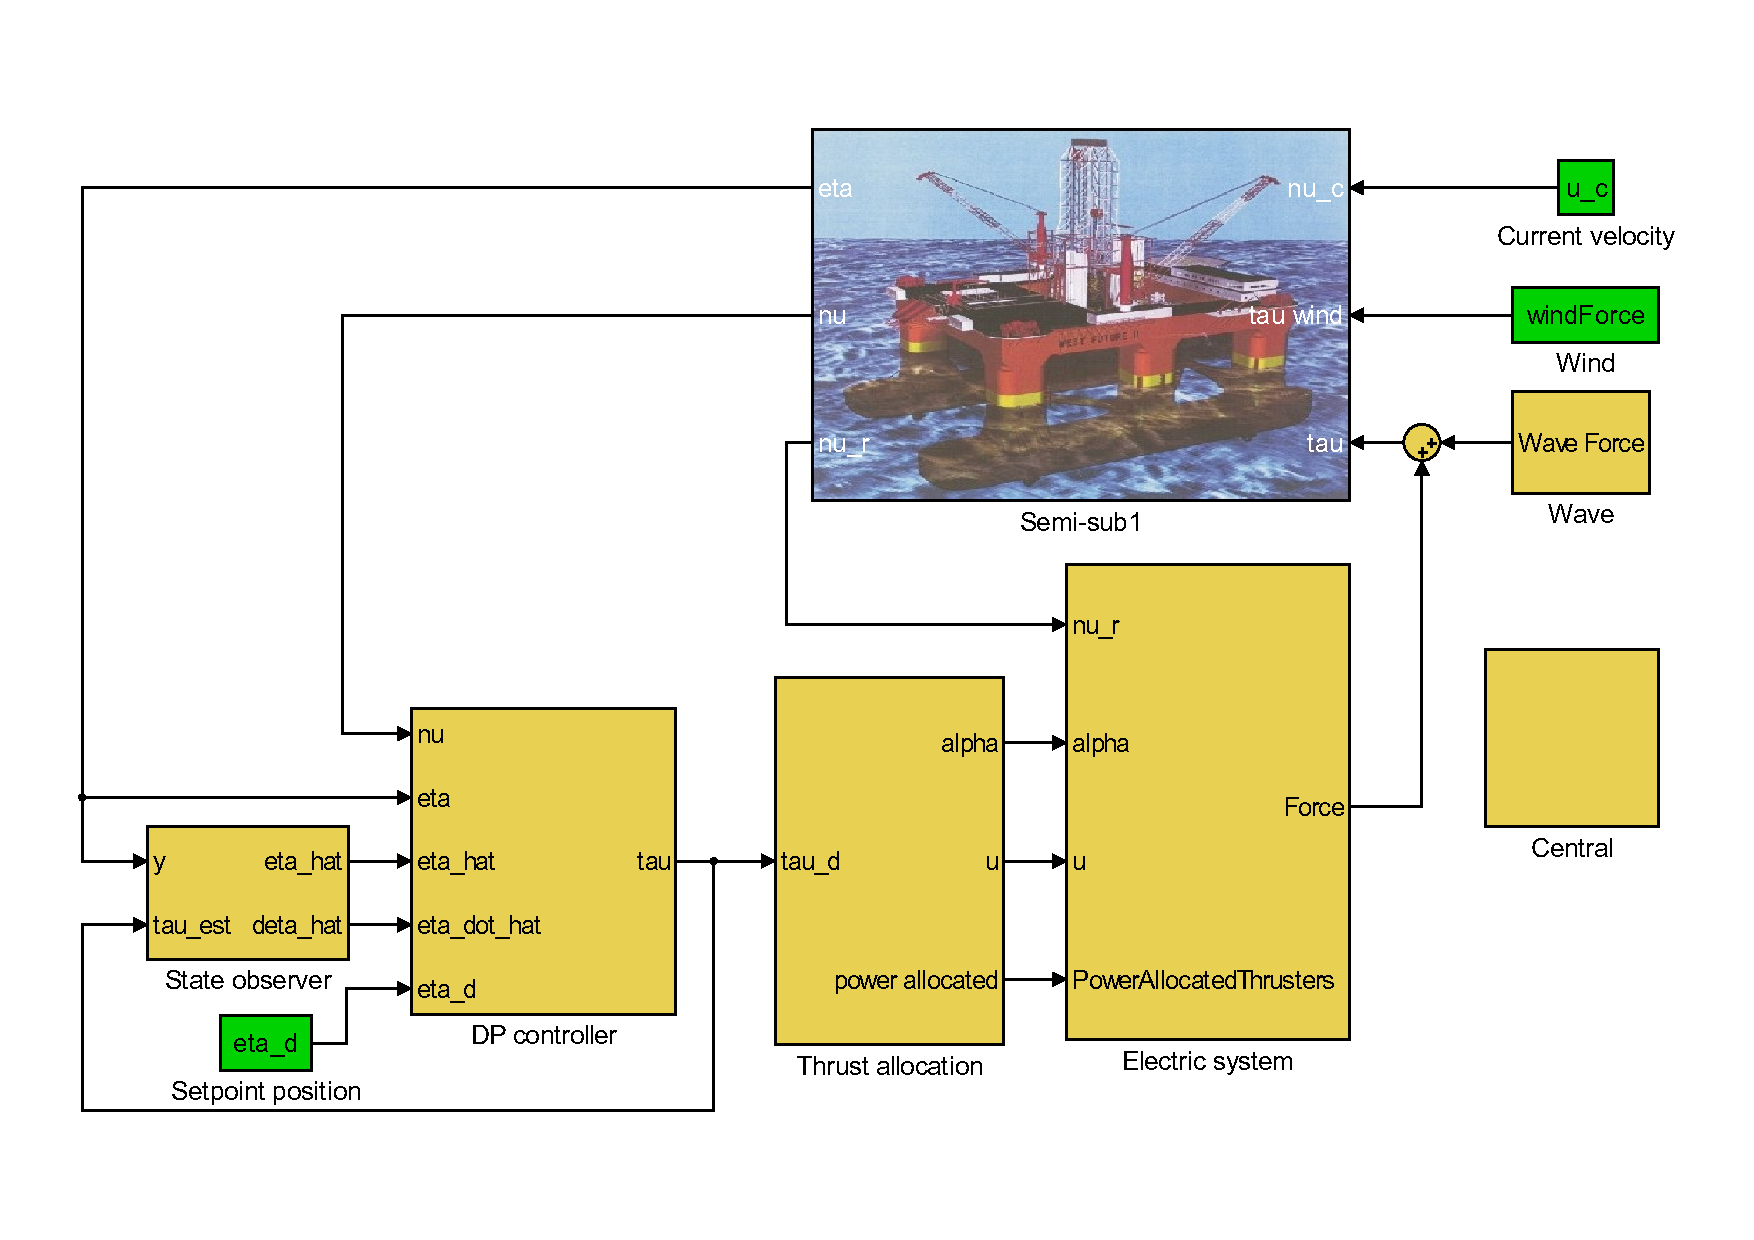
\includegraphics[trim=30 60 30 60,width=.7\textwidth,clip]{./figures/DPscheme}
\caption{Example of top level view, including the vessel model, observer, DP~controller, thrust~allocation, and the~electrical~system.
The electrical system is further presented in Fig.~\ref{fig:PowerPlantsscheme}.
The central block is used for common calculations.}
\label{fig:DPscheme}
\end{figure*}

For this case, the view contains:\begin{enumerate}
\item Observer; estimates the position and velocity of the vessel from measurements.
\item DP control system; calculates a desired thrust command.
\item Thrust allocation (TA); converts the desired thrust command for the vessel to thrust commands for each thruster.
\item Electric system with thruster model; converts the thrust command to actual thrust, and electric power plant.
\item Environmental model; generates realistic loads for the environment.
\item Vessel model; calculates the motions of the vessel given the thruster and environmental loads.
\item Central; this is a block used for common calculations.
\end{enumerate} 

The electric power plant is modeled inside the electric system block.
An example power plant is shown in Fig.~\ref{fig:PowerPlantsscheme} and consists of:
\begin{enumerate}
\item Generator set; consisting of a prime mover (e.g., diesel engine), a generator, a speed governor, and an automatic voltage regulator (AVR).
\item Thruster drives; consisting of a frequency converter, an electric motor, a propeller, and controller.
\item Other components; This can be hotel and drilling loads, which are modeled as time series of power consumption. However, this block may also be used for energy storage, such as batteries with a frequency converter. The load is then negative when the block delivers power and positive when it consumes power.
\item Switchboards; connecting loads and producers.
\item Breakers; connecting and disconnecting components.
\end{enumerate}


\begin{figure*}[t!]
\centering
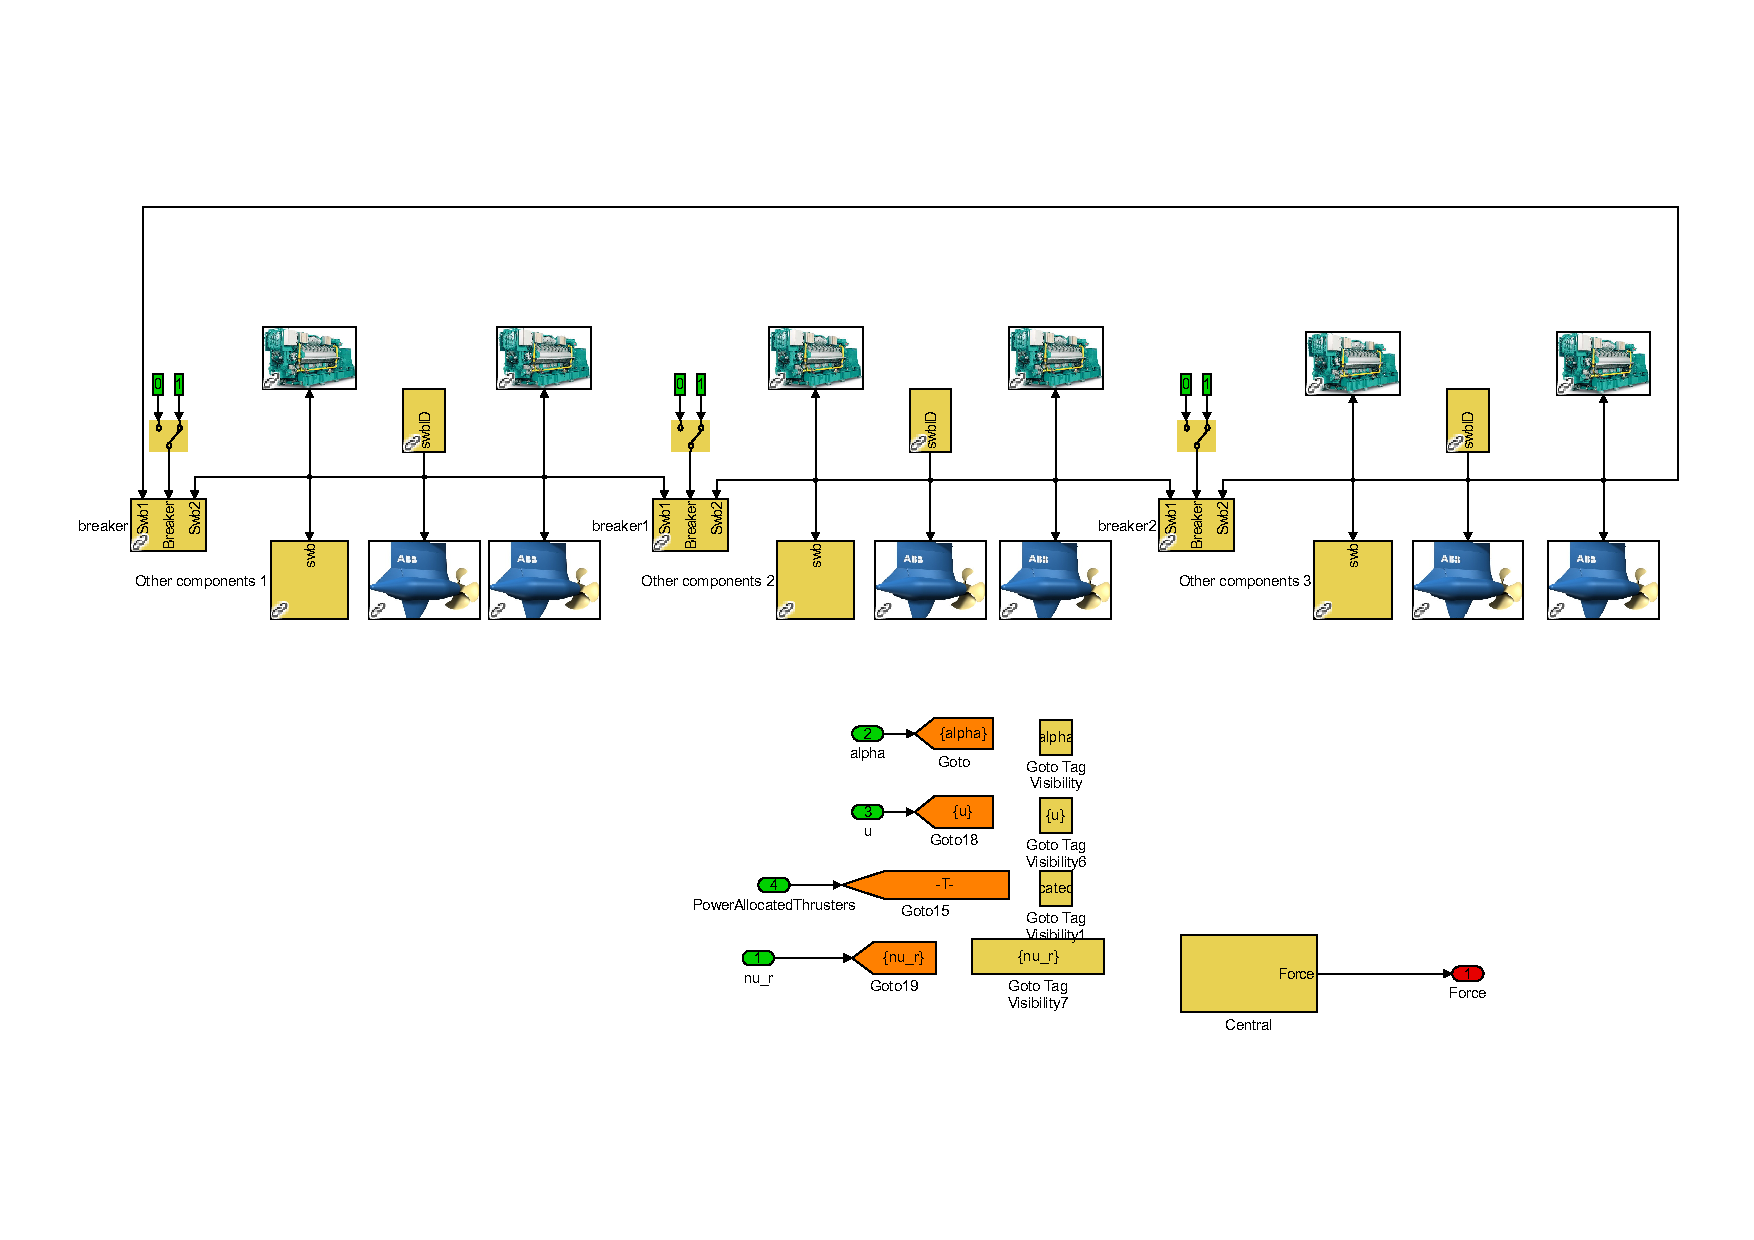
\includegraphics[trim=30 280 30 80,width=\textwidth,clip]{./figures/elscheme.pdf}
\caption{Example of power plant view, including the bus tie breakers, thrusters, generator sets, and other loads block. }
\label{fig:PowerPlantsscheme}
\end{figure*}



Simulink was chosen in order to extend MSS~toolbox~\cite{MSS} to include better thruster models and an electric power plant.
The downside by choosing Simulink is the modeling of interconnections.
The system is hard to divide into levels as required by the subsystem architecture of Simulink.
We chose to use the top level model view for the vessel control, further the electric power plant is a subsystem in this view.
The electric power plant is made to mimic a single line diagram.
%However, no information other than the configuration is sent via the lines in Simulink.
%Goto blocks are used to send information between the blocks to avoid a ``spagetti'' diagram with too many lines.
%A script is used to automate the configurations of the goto blocks.
The stiff solver ode15s is used as numerical solver in the case study, since the local controllers give a stiff model.
When the simulation is done on a National Instrument cRIO for real time simulations, the solver ode3 with 1~millisecond steps is used, since cRIO does not support variable timestep solvers.

Some first order lowpass filters are used to avoid algebraic loops, where the time constant of the filters are chosen to be smaller than the fastest dynamics of the relevant models.
This is needed since we ignore some fast dynamics.
The filters can therefore be seen as simplified models of the ignored dynamics.
One example is the power available signal.
An algebraic loop occurs since the power available is dependent on the power consumption, while the power available also constraints the power consumption.
This is solved by adding a lowpass filter on the power available signal, which is faster than the time scale of the consumers.
This may also be solved by using discrete time for these signals.
However, this reduces the performance of the chosen implicit ode solver.

\subsection{Time Scales}
The time scale of the listed use cases is in order of seconds to minutes.
However, parts of the dynamics of a marine power plant is much faster than 1 second.
In Fig.~\ref{fig:TimeScale}, the time scale of the simulator components are shown.
This shows that some dynamics can be ignored by model reduction.
This is the case for most of the elements of the electric system. 
Further discussion of the time scales are given later, in each model components section.

\begin{figure}
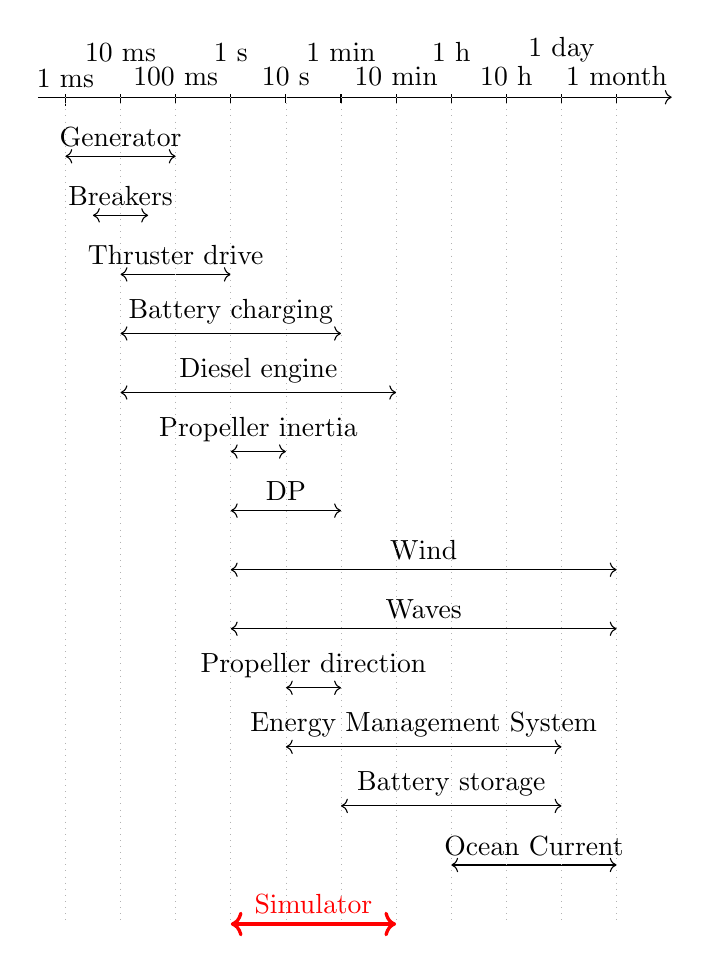
\begin{tikzpicture}[y=.5cm, x=.7cm]
\newcommand{\extraVertical}{4mm}%
\newcommand{\normalVertical}{1mm}%
\newcommand{\nodeVSkip}{-1.5}%
\newcommand{\element}[4]{\draw[<->]  ($ (a)+(#2,#1*\nodeVSkip)$) -- +(#3,0) node[midway,above] {#4}; 
}
\draw[->] (.5,0) -- coordinate (x axis mid) (12,0) ;
\draw (1,1pt) -- (1,-3pt)   node[above=\normalVertical] {1 ms};
\draw (2,1pt) -- +(0,-3pt) node[above=\extraVertical] {10 ms};
\draw (3,1pt) -- +(0,-3pt) node[above=\normalVertical] {100 ms};
\draw (4,1pt) -- +(0,-3pt) node[above=\extraVertical] {1 s};
\draw (5,1pt) -- +(0,-3pt) node[above=\normalVertical] {10 s};
\draw (6,1pt) -- +(0,-3pt) node[above=\extraVertical] {1 min};
\draw (7,1pt) -- +(0,-3pt) node[above=\normalVertical] {10 min};
\draw (8,1pt) -- +(0,-3pt) node[above=\extraVertical] {1 h};
\draw (9,1pt) -- +(0,-3pt) node[above=\normalVertical] {10 h};
\draw (10,1pt) -- +(0,-3pt) node[above=\extraVertical] {1 day};
\draw (11,1pt) -- +(0,-3pt) node[above=\normalVertical] {1 month};
\coordinate (a) at (1,\nodeVSkip);
\element{0}{0}{2}{Generator}
\element{1}{.5}{1}{Breakers}
\element{2}{1}{2}{Thruster drive}
\element{3}{1}{4}{Battery charging}
\element{4}{1}{5}{Diesel engine}
\element{5}{3}{1}{Propeller inertia}
\element{6}{3}{2}{DP}
\element{7}{3}{7}{Wind}
\element{8}{3}{7}{Waves}
\element{9}{4}{1}{Propeller direction}
\element{10}{4}{5}{Energy Management System}
\element{11}{5}{4}{Battery storage}
\element{12}{7}{3}{Ocean Current}
\draw[red,<->,very thick] ($(a)+(3,13*\nodeVSkip)$) -- +(3,0) node[midway,above] {Simulator};
\newcommand{\heightFigure}{14*\nodeVSkip}%
\foreach \x in {1,2,...,11} {
	\draw[very thin,dotted,black!30] (\x,0) -- +(0,\heightFigure);
}

\end{tikzpicture}
\caption{List of components in the simulator and their time scales.}
\label{fig:TimeScale}
\end{figure}



\subsection{Power Management System}
The PMS objective is to make sure there is always enough power available, to prevent blackout.
If a blackout occurs, the PMS should restore the power as fast as possible.
The PMS starts additional generators when the excessive power capacity of the connected producers is too small.
In addition, the PMS allocates power to the different consumers.
This is done by first summing the current power capacity of the producers.
This is then shared among the consumers based on their desired power consumption and priority.
A signal, called \textit{power available}, is sent to some consumers, stating the maximum power limit for the specific load.
Load shedding (disconnection of consumers) is done in extreme cases, when power reduction must be done immediately (e.g., close to underfrequency).

Fast load reduction is an alternative method to reduce the power consumption quickly.
It reduces the load of the thruster drives, since they can change the power consumption quickly due to the frequency converters.
Shortly after the fault is cleared or the capacity is increased, the drives can increase their loads.
This is in contrast to load shedding where the consumers often needs to be restarted after being disconnected.

The PMS will also adjust the droop and isochronous load sharing parameters to adjust the load sharing.
This is done during progressive loading after connection of generator sets.
Progressive loading is implemented to ensure that the power generation of the new producer is slowly increased from no load to desired load sharing.

The PMS algorithm is implemented in~C++ as an S-function block and can easily be configured to different power plants.
The object oriented focus of the simulator is kept in the PMS implementation, so that new functionalities, such as automatic start and stop, easily can be added.

%The PMS updates at 10 Hz, which is within the desired time scale of the simulator.

\subsection{Bus Voltage Calculation}
\label{sec:voltage}
The voltage of the bus is needed to calculate the load sharing of the generators.
The generators are connected in parallel as shown in Fig.~\ref{fig:circuitbus}.
The loads are assumed to be independent of the bus voltage, their active and reactive power are therefore given.
Th\'{e}venin equivalent circuit of the connected generator sets is used to calculate the bus voltage, as shown in Fig.~\ref{fig:circuitThevenin}.
This circuit is closed by the loads, which have a known power consumption but unknown impedance.

\begin{figure*}
\centering
\subfloat[ ]{
\centering
\begin{circuitikz}[american voltages]
\draw
(0,0) to [short] (6.5,0)
to [sV, l_=$\tilde{E}_{a,n}$] ++(0,1.5)
to [R, l_=$Z_n$] ++(0,1.5)
to [short, i_=$\tilde{I}_{a,n}$] ++(0,1)
to [short] (0,4)
(0,0) to [vR, l_=$Z_\mathrm{load}$] (0,4)

(4,0)  to [sV, l_=$\tilde{E}_{a,2}$] ++(0,1.5)
to [R, l_=$Z_2$] ++(0,1.5)
to [short, i_=$\tilde{I}_{a,2}$] ++(0,1)

(2,0)  to [sV, l_=$\tilde{E}_{a,1}$] ++(0,1.5)
to [R, l_=$Z_1$] ++(0,1.5)
to [short, i_=$\tilde{I}_{a,1}$] ++(0,1)
node (A) at (-.25,0) {}
node (B) at (-.25,3.5) {}
(A) to [open, v^>=$\tilde{V}$] (B);
\node at (5.25,2) {...};
\end{circuitikz}
\label{fig:circuitbus}
}
\subfloat[ ]{
\centering
\begin{circuitikz}[american voltages]
\draw
(0,0) to [short] (3,0)
to [sV, l_=$\tilde{E}_{T}$] ++(0,1.5)
to [R, l_=$Z_T$] ++(0,1.5)
to [short, i_=$\tilde{I}$] ++(0,1)
to [short] (0,4)
(0,0) to [vR, l_=$Z_\mathrm{load}$] (0,4)
node (A) at (-.25,0) {}
node (B) at (-.25,4) {}
(A) to [open, v^>=$\tilde{V}$] (B);
\end{circuitikz}
\label{fig:circuitThevenin}
}
\caption{(a) Circuit diagram of bus with one load with the impedance $Z_\mathrm{load}$ and $n$ generators. (b) Thevenin equivalent circuit of~(a).}

\end{figure*}
This gives the equation 
\begin{equation}
P_{bus}+j Q_{bus} = 3 \tilde{V} \tilde{I}^* = 3 \tilde{V} \frac{\tilde{E}^*_T-\tilde{V}^*}{Z_T^*},
\label{eq:powerBus}
\end{equation}
where $P_\mathrm{bus}$ and $Q_\mathrm{bus}$ are the active and reactive power of the loads, $\tilde{V}$ is the line-to-neutral bus voltage, $\tilde{I}$ is the current, $\tilde{E}_T$ is the Th\'{e}venin equivalent voltage, and $Z_T$ is the Th\'{e}venin equivalent impedance.
Equation~\eqref{eq:powerBus} has either two solutions, one solution, or no solution.
For the case where there exists two solutions, the solution with the largest absolute value for the bus voltage is used.
The largest voltage yields a high resistance of the load, and a low current, hence low internal loss.
The lower voltage solution gives a resistance smaller than the Th\'{e}venin equivalent resistance, which is unphysical.
This yields a high current, with very high internal loss since most of the voltage drop occurs over the internal impedance.

During simulations it may occur that there exists no valid solution. This may happen when the load increases rapidly (a load is connected) or the Th\'{e}venin equivalent voltage of the generator decreases rapidly (fault in AVR or disconnection of a generator).
In such cases, the voltage is set to a low value.
This gives an incorrect load sharing, but the AVR will increase the voltage quickly.
During the verification study in Section~\ref{sec:elverification}, a valid solution of the bus voltage was regained within 0.1~millisecond.
This is permissible since the time is very short compared to the time scale of the mechanical system.
A lowpass filter must therefore be added when simulating voltage protection relays.

\subsection{Generator}
\label{sec:Generator}
In marine power plants, synchronous generators are typically used to produce power.
As earlier mentioned, the generator is assumed to be in steady state and with balanced phases.
The electrical torque is 
\begin{equation}
\tau_{e} = \dfrac{p+p_\mathrm{loss}}{\omega} = \dfrac{p}{\omega}+\dfrac{r(p^2+q^2)}{\omega v^2},
\end{equation}
where $p_\mathrm{loss}$ is the power loss in the generator, $r$ is the resistance in the stator windings, $q$ is the reactive power, and $v$ is the terminal voltage.
The terminal line-to-neutral voltage is given as~\cite{Krause2013}:
\begin{equation}
\tilde{V}_a=-Z \tilde{I}_a+\tilde{E}_a,
\end{equation}
where $Z$ is the internal impedance of the generator set, $\tilde{I}_a$ is the current through phase $a$ and $\tilde{E}_a$ is the induced line-to-neutral voltage for phase $a$.

It is assumed that the magnitude of $\tilde{E}_a$ is perfectly controlled by the AVR or at least the dynamics are much faster than the dynamics of the mechanical system.
This is verified in Section~\ref{sec:elverification}.
The per phase angle of $\tilde{E}_a$ is
\begin{equation}
\angle{\tilde{E}_a} = \frac{\theta N_\mathrm{poles}}{2},
\end{equation}
where $N_\mathrm{poles}$ is the number of poles of the generator.

The AVR regulates the terminal voltage by manipulating the induced voltage.
In this simulator we use a droop controller to determine the set-point, based on the reactive power of the generator set.
This takes care of the reactive load sharing. 
The generators deliver equal amount of reactive power if they have equal voltage droop curves.



\subsection{Diesel Engine}
\label{sec:dieselengine}
The dynamics of the diesel engine are the slowest dynamics of a diesel electric power plant. 
Most modern diesel engines are turbocharged to provide increased power density. 
When a turbocharged diesel engine needs to increase its delivered power, more air is required into the cylinders to avoid incomplete combustion and visible smoke in the exhaust.
However, the response of the air system is rather slow, due to the rotating inertia of the turbocharger and the large air- and exhaust receiver volumes, which gives rise to the \textit{turbo-lag}.
In addition, increasing the fuel injection rises the temperature in the cylinder.

Constraints are, therefore, added to the engine control output by the engine manufacturer to ensure that the fuel injection is not changed too quickly.
This is done to avoid that the engine is damaged by a rapid change of temperature, and that the air pressure in the inlet manifold is large enough to allow for a complete combustion. 
These constraints are in some cases conservative and the air dynamics may be neglected since the engine will always run with complete combustion due to these constraints.

Transients of the diesel engines can be grouped into three categories~\cite{Benajes2002}. 
The first is energy transfer delay which happens due to signal delay, preset valve closure or injection timing. 
The time scale of such phenomena is in milliseconds. 
In simulation, this can only be seen by detailed modeling of cylinder process and fuel injection system. 
Secondly, the already mentioned air dynamics are the most interesting physics in this kind of application. 
The typical transient time scale of the air dynamics is in seconds. 
Lastly, thermal transient is caused by the thermal inertia of the system, which may have time scale of tens of minutes. 

\subsubsection{Mean Value Model}
The main purpose of the diesel engine simulation model is to capture the air dynamics including pressure before the engine cylinder which can be related to the charge air available for combustion. 
In the mean value engine model, most of the physics in the engine system components are captured except for the in-cylinder process, i.e., the thermodynamic cycle. 
The main components included in the model are an engine cylinder block, a turbocharger, a charge air cooler, an air receiver and an exhaust receiver. 
The implemented mean value engine model is based on the models presented in~\cite{Guzzella2010,Chow1999,Heywood1988,Zacharias1967,Yum2013,Pedersen2000}.

The engine system including a turbocharging system is inherently a thermodynamic process with gas mixture as medium. Therefore, main variables of the system are pressure, $p$; temperature, $T$; and fuel-air equivalent ratio, $F$. Also flow variables, such as mass flow of gas, $\dot{m}$;  enthalpy flow or rate of change in internal energy, $\dot{E}$; and mass flow of burned fuel, $\dot{m}_\mathrm{b}$, are necessary in order to describe the dynamics of the system. 

A filling and empty method \cite{Chow1999} is used to construct the thermodynamic process model of the system. In this approach, the target model is constructed by placing control volumes in a series as configured in the real system and putting a flow restriction between adjacent control volumes. 
It is assumed that the thermodynamic states, such as pressure and temperature, are uniform within in a control volume and that there is no accumulation of mass in the flow restriction.
Then, all the components fall into two categories: a thermodynamic control volume or a flow restriction. 
Generally, pipes, receivers and cylinders are thermodynamic control volumes; whereas any valve, port, compressor, turbine and heat exchangers are considered as flow restrictions. 

Thermal control volumes determine the thermodynamic states of the system. They consist of two parts. The first one is a flow junction where mass conservation and the first law thermodynamics are implemented. The second part is the flow accumulation where the net rate of change in mass and energy are integrated. The integrated values are the mass, $m_{\mathrm{cv}}$; the internal energy, $U_{\mathrm{cv}}$; and mass of burned fuel within the control volume, $m_{\mathrm{f}}$; which are states of the system. Pressure and temperature are derived from a table of thermodynamic properties, such as the JANAF table~\cite{Chase1998}, and by using the equation of state (i.e. ideal gas law). In order to achieve faster simulations, a semi-empirical formula for thermodynamic properties found in~\cite{Zacharias1967} is used in place of the table. 

A flow restriction, placed between two control volumes, determines the flow rate of mass and energy between them. The flow rate depends on pressure and temperature of the adjacent control volumes. In many cases, the equations of the equivalent ideal flow for compressible gas is used for this purpose. The equation used for the model is given in \cite{Heywood1988}. The equation, however, assumes an isentropic process across the restriction. Therefore, any forms of energy gain or loss should be accounted in order to achieve the conservation laws. 

In case of a compressor and a turbine, the model requires a performance data map from measurement or a manufacturer. The map represents the relationship between the pressure ratio across the device and rotating speed of the rotor, $\omega_\mathrm{TC}$; versus the corrected mass flow, $\dot{m}_{\mathrm{corr,TC}}$; and the isentropic efficiency of the process, $\eta_{\mathrm{TC}}$. Having acquired the mass flow and the efficiency, the energy flow in and out can be calculated assuming an isentropic process. Then the torque for each turbomachine can be calculated as
\begin{equation}
\tau = \frac{\dot{m} \Delta h}{\omega_\mathrm{TC}}
\end{equation}
where, $\dot{m}$ and $\Delta h$ is actual mass flow and change in enthalpy, respectively, across the machine.
A dynamic equation is used for the mechanical rotation of the turbocharger.
\begin{equation}
J\dot{\omega} = \tau_{\mathrm{turb}} - \tau_{\mathrm{comp}},
\end{equation}
where $\tau_{\mathrm{turb}}$ and $\tau_{\mathrm{comp}}$ are the torque by the turbine and compressor, $J$ is the rotational inertia of the turbocharger, and $\omega$ is the angular velocity of the turbocharger.

The whole engine block, including intake and exhaust valves, fuel injection system, cylinders and pistons is simplified to a single flow restriction model. 
In this model, the input is the pressure, $p_{\mathrm{AR}}$; and temperature of the air receiver, $T_{\mathrm{AR}}$; the engine speed, $\omega_\mathrm{eng}$; and the fuel rack position, $u$. Mass flow through this restriction model can be determined given a known volumetric efficiency of the process, $\eta_\mathrm{vol}$. 
\begin{equation}
\begin{aligned}
{{\dot m}_\mathrm{in}} &= {\eta _\mathrm{vol}}\left( {{p_\mathrm{AR}}} \right)  {\rho _\mathrm{AR}}{V_d}\frac{{{\omega _{{\mathrm{eng}}}}}}{{n_s \pi }}, \\
{{\dot m}_\mathrm{out}} &= {{\dot m}_\mathrm{in}} + {{\dot m}_{b}}, \\
{{\dot m}_{b}} &= {m_{f,\max }} u \frac{{{\omega _{{\mathrm{eng}}}}}}{{n_s \pi }} ,
\end{aligned}
\end{equation}
where $\rho_\mathrm{AR}$ is the density of the gas in the air receiver, $n_s$ is the number of stroke of the engine cycle, and ${m_{f,\mathrm{max} }}$ is the maximum amount of fuel injected per cycle.
Energy flow in and out of the cylinder is also calculated as follows
\begin{equation}
\begin{aligned}
{{\dot E}_\mathrm{in}} &= {{\dot m}_\mathrm{in}}{h_\mathrm{AR}}\left( {{p_\mathrm{AR}},{T_\mathrm{AR}}} \right), \\
{{\dot E}_\mathrm{out}} &=  \dot E_\mathrm{in}+ {{\dot m}_{b,\mathrm{out}}}LHV\left( {1 - {C_{HT}} - \frac{1}{{\mathrm{LHV} \cdot \mathrm{SFC}}}} \right),
\end{aligned}
\end{equation}
where $h_\mathrm{ar}$ is the enthalpy of air from air reciever volume, $LHV$ is low heating value of the fuel and $C_{HT}$ is the heat transfer ratio and $SFC$ is the specific fuel consumption. 
The torque output of the engine is
\begin{equation}
 = \frac{\dot{m}_{b,out}}{ \omega _\mathrm{eng} \cdot \mathrm{SFC} }.
\end{equation}

The overall mean value engine system model is presented in Fig.~\ref{fig:MVEMscheme}.
Both compressor and turbine model require ambient pressure and temperature as boundary conditions for the system. The input to the overall model is fuel rack position and engine speed; the output is pressure and temperature of the air receiver, volumetric efficiency, and torque.
The first three outputs are used in order to calculate the mass trapped in the cylinder per cycle, which is further used to calculate the maximum allowable injected fuel amount according to given fuel-air equivalent limit. This functionality is termed as smoke limiter. 
The smoke limiter ensures that the charge in the cylinder is lean enough to avoid visible smoke during rapid power output increase. 
\begin{figure}
\normalsize
\centering
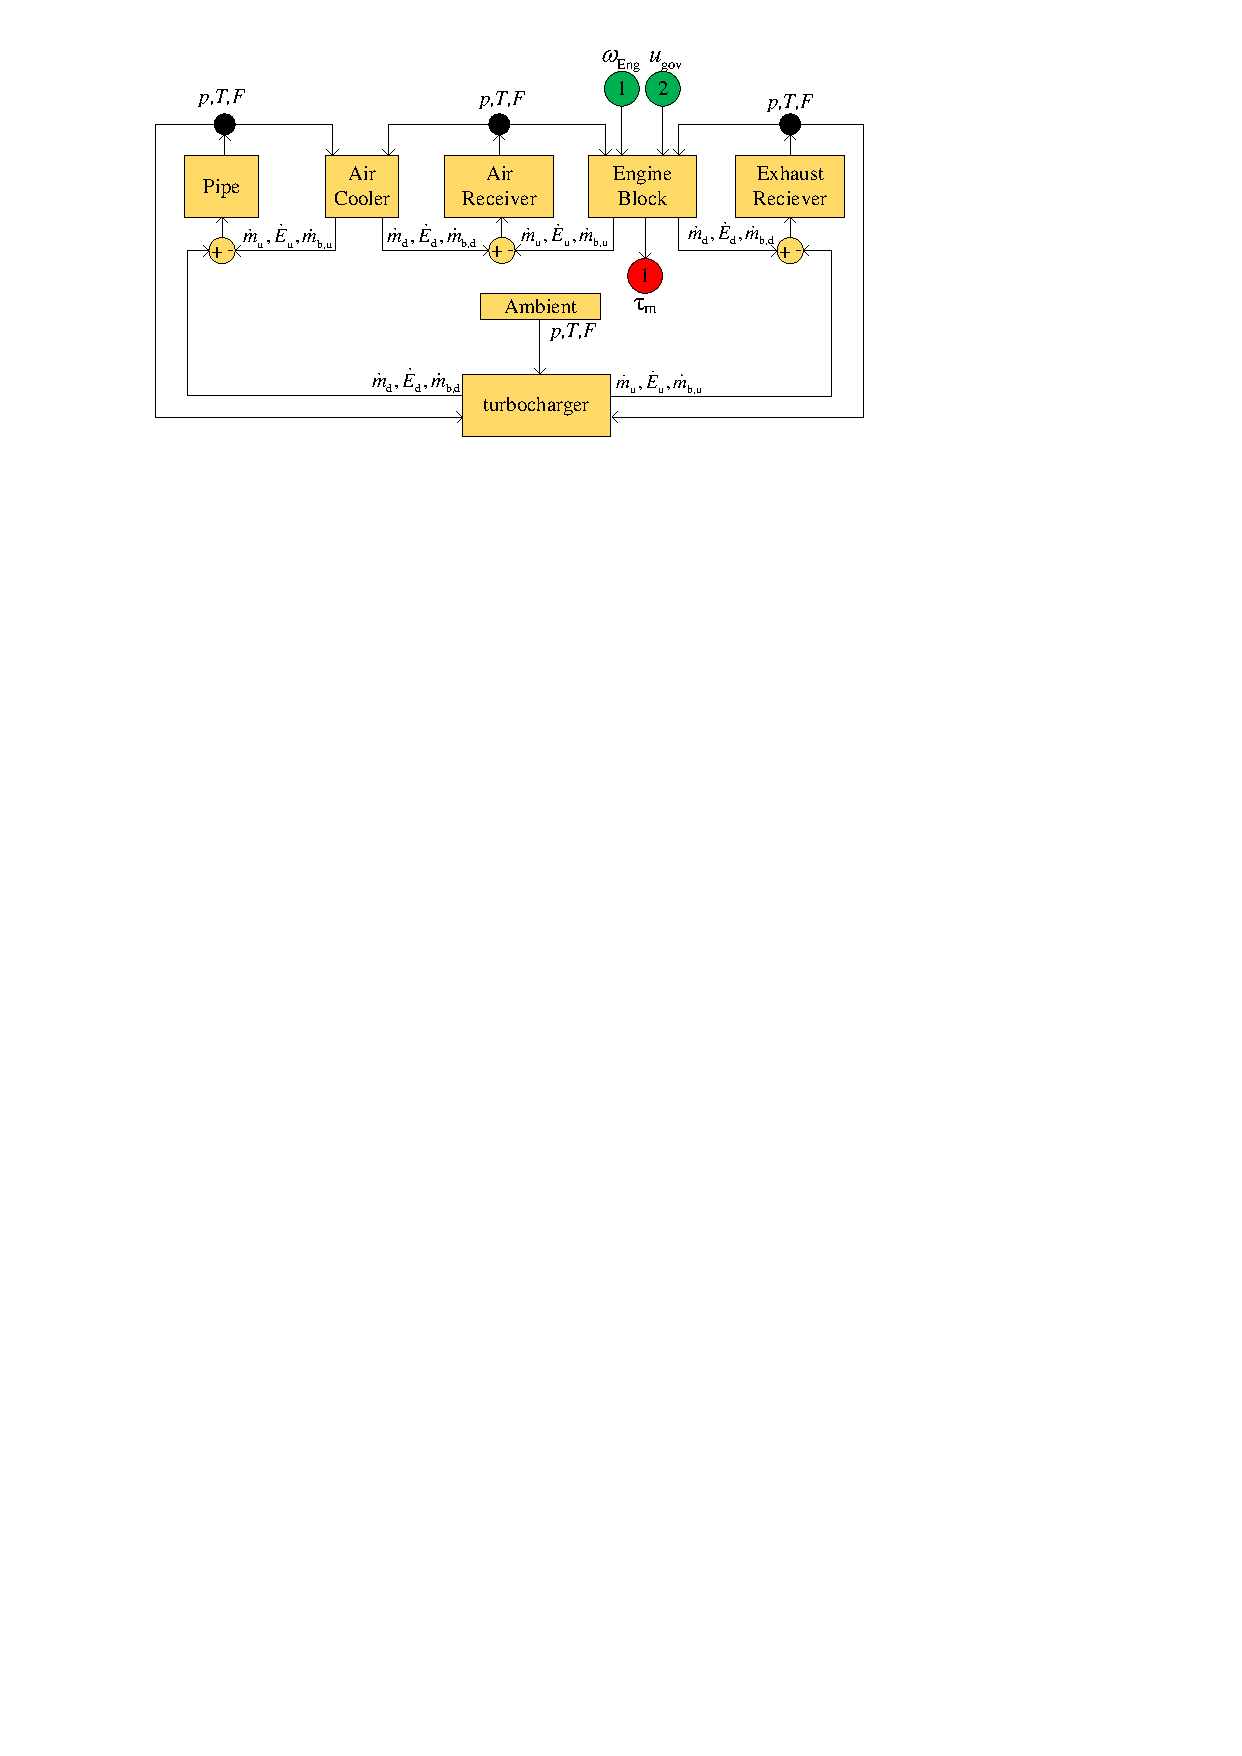
\includegraphics[width=\columnwidth,trim=2.75cm 22.5cm 6.5cm 0.8cm]{./figures/MVEMScheme.pdf}
\caption{Mean value engine system model scheme, including a turbocharger, a charge air cooler and incylinder process.}
\label{fig:MVEMscheme}
\end{figure}

A short-coming of such a model is that it requires extensive parameter identification in order to achieve reasonable accuracy. However, a well-defined engine model can be used for different cases if the main physical variables are converted into per unit values. This may cause inaccurate response characteristics since machines at a various power range should have somewhat different time scales. If it is possible to find the response characteristics of a genset to step load changes, the overall model including the governor can be re-tuned to match the given characteristics. Such characteristics can be found in the manufacturer's documentation, e.g. ~\cite{MANEnginesandSystems2013}.

\subsubsection{Rate Constrained Model}
A simplified model can be used for engines where the fuel rate is constrained such that the combustion is complete.
In Sec.~\ref{sec:dieselconstraints}, simulations show that this is the case for maritime engines, due to the conservative rate constraints set by the engine manufactures.
A simplified model which ignores the air dynamics and requires only one parameters can therefore be used.
\begin{equation}
\tau_m = k_u u, 
\end{equation}
where $\tau_m$ is the torque output of the diesel engine and $k_u$ is the gain from fuel rate to mechanical torque.

\subsubsection{Shaft Speed Dynamics}
The engine shaft speed dynamics is given by
\begin{align}
\dot{\theta} =& \omega \omega_b,\\
\dot{\omega} =& \frac{1}{2H} \left(-D_f \omega + \tau_m  - \tau_e \right),
\end{align}
where $\theta$ is the mechanical angle, $\omega$ is the per unit mechanical angular velocity, $\omega_b$ is the base mechanical angular velocity, and the windage friction constant is denoted $D_f$.
This is derived by the swing equation and assuming linear damping.
H is defined as
\begin{equation}
H = \dfrac{1}{2}\dfrac{J \omega_b^2}{P_b},
\end{equation}
where $J$ is the rotational inertia of the generator set and $P_b$ is the base power of the generator set~\cite{Krause2013}.

\subsubsection{Governor}
The two engine models use the same governor, which is based on droop control~\cite{Woodward2004}.
The commanded fuel index is then calculated by a PID controller with back calculation to avoid wind-up of the integrator term.
The derivative of the frequency is calculated by using the \textit{dirty derivative}.
\begin{align}
&\omega_\mathrm{ref} = \omega_\mathrm{NL}-K_\mathrm{droop}p, \\
&u = K_p (\omega_\mathrm{ref}-\omega)+K_i \xi - K_d \hat{\dot{\omega}},\\
&\dot{\xi} = \omega_\mathrm{ref}-\omega + K_b(u_\mathrm{saturated}-u),\\
&\hat{\dot{\omega}}= N(\omega-\hat{\dot{\omega}}),
\end{align}
where the $K_d$, $K_i$, and $K_p$ are the derivative, integration, and proportional gain. The produced power in per unit by the generator is denoted $p$. The symbols $\omega_\mathrm{ref}$, $\omega_\mathrm{NL}$, and $\hat{\dot{\omega}}$ are the reference frequency, set-point frequency at zero active power, and estimated time derivative of the frequency.

For the rate constraint model, additional constraint on the fuel index is needed to avoid too large temperature variations in the cylinder and sooting due to too little air for complete combustion. This constraint is predefined and, therefore, static. In the case study, the engine is allowed to increase the fuel index with 20\% of the rated output and then increase the fuel index with $8.1 \%/s$. This is found by tuning the engine model response to best fit recovery time and frequency drop given in \cite{MANEnginesandSystems2013}.

For the mean value model, a smoke limiter constraints the governor's command. 
The amount of air available for a cycle is
\begin{equation}
\label{eq:airAvail}
m_\mathrm{air} = \eta_\mathrm{vol}\frac{p_\mathrm{rec}V_{D}}{RT_\mathrm{rec}} ,
\end{equation}
where $\eta_\mathrm{vol}$ is the volumetric efficiency, $p_\mathrm{rec}$ and $T_\mathrm{rec}$ are the pressure and temperature at an air receiver, $R$ is the specific gas constant and $V_D$ is the displacement volume of a cylinder.
Given the maximum fuel-air equivalent ratio, $F_\mathrm{max}$, the maximum fuel index, $u_\mathrm{max}$, is given by
\begin{equation}
\label{eq:maxFIndex}
u_\mathrm{max} = \eta_\mathrm{vol}\frac{p_\mathrm{rec}V_{D}}{RT_\mathrm{rec}} \frac{F_\mathrm{max}f_s}{m_\mathrm{f,inj}},
\end{equation}
where $f_s$ is the stoichiometric fuel-air ratio and $m_\mathrm{f,inj}$ is the amount of maximum fuel injection per cycle. In the case study, the $F_\mathrm{max}$ is chosen as 1 in order to give a reasonable engine response.


\subsection{Energy Storage Devices}
ESD include batteries, capacitors, fuel cells or any other device capable of providing and consuming power on demand. They are accounted on the PMS as available power reserve and depending on the control strategy adopted by the PMS, it might substitute fast load reduction strategy. The inner dynamics in the energy storage devices is disregarded, since it is assumed that its dynamics are much faster than the remaining components.

All components included here are a simplified, since the losses are modeled using an efficiency table. This method makes it simple to include and model more components with data provided by the manufacturers.


\subsection{Thrusters}
The thrusters are modeled as propellers which are driven by electrical motors.
The propellers are assumed to be fixed pitch, while the speed is variable.
No thruster-thruster or thruster-hull interaction losses are included, as these are generally hard to describe.
It is assumed that the torque of the electrical motor is perfectly controlled.
A frequency controller is often used to control the motor.
The time scale of the dynamics of the frequency converter is much faster than the dynamics of the mechanical part of the thruster drives, and can therefore be neglected.
A speed controller is used to control the thrust. 
The open water characteristics are used to calculate the desired shaft speed, from the requested thrust.
The thrust is assumed to be~\cite{Sorensen2013}
\begin{equation}
T_a = \operatorname{sign}(n)K_T \rho D^4 n^2,
\end{equation}
where $K_T$ is the thrust coefficient found from open water tests, $\rho$ is the density of water, $D$ is the propeller diameter, and $n$ is the shaft speed.
This gives the desired shaft speed
\begin{equation}
n_d = \operatorname{sign}(T_d) \sqrt{\frac{|T_d|}{K_T \rho D^4}}.
\end{equation}

The desired thrust signal must be smoothed since the desired thrust is typically calculated at 1~Hz.
Large power fluctuation will occur at each thruster command update instant if this is not done.
A second order filter is therefore used for this task.

The four-quadrant model of the propeller presented in~\cite{Smogeli2006}, is used to calculate the actual thrust and torque of the thruster.
The benefit of this model is that it models \textit{wind milling} (i.e., shaft speed and torque have different signs).
The advance velocity of the propeller is assumed to be equal to the relative velocity of the vessel.
This means that wave-propeller interaction due to vessel motion is included, but wave-propeller interaction due to wave induced particle motion is not included~\cite{Sorensen2009}.

This model was first presented by~\cite{Miniovich1960}. 
The thrust and torque coefficients are defined as
\begin{align}
C_T =& \frac{T_a}{\frac{1}{2}\pi R^2 \rho V_{0.7}^2}, \; \mathrm{and} \\
C_Q =& \frac{Q_a}{\frac{1}{2}\pi R^3 \rho V_{0.7}^2},
\end{align}
where $T_a$ is the thrust, $R$ is the radius of the propeller, and $Q_a$ is the propeller torque. $V_{0.7}$ is the undisturbed incident velocity to the propeller blade at radius $0.7R$ and is defined as
\begin{equation}
V_{0.7}=\sqrt{V_a+(0.7\omega R)^2},
\end{equation}
where $\omega$ is the angular velocity of the propeller shaft.

The angle of attack of the propeller at $0.7R$, $\beta$, is defined as
\begin{equation}
\beta = \arctan\left(\frac{V_a}{0.7 \omega R}\right).
\end{equation}
To estimate $C_T$ and $C_Q$, a Fourier approximation as a function of $\beta$ is used, with parameters from~\cite{Smogeli2006}.

The power consumption of the thrusters are typically reduced after a fault by the fast load reduction.
This is done by limiting the torque of the electrical motor driving the propeller.
In practice, this is done by the frequency converter.

The thrust allocation needs an estimate of the power consumption of the thrusters.
The forth quadrant model is not suitable for this purpose, as the advanced velocity is not available for the thrust allocation.
The power consumption by the electric thruster is therefore approximated by
\begin{equation}
p = K_{f2p} |f|^{1.5},
\end{equation}
where $f$ is the thrust amplitude, and $K_{f2p}$ is a constant.
Due to the approximation, the actual and approximated power consumption may be different.
%This means that the power consumption constraints may be violated even though the solution satisfies the power constraint.
%The thrusters are therefore given a power constraint based on the approximated power consumption in the thrust allocation.
%This ensures that the thrusters do not use more power than available for the DP on each of the buses.


\subsection{Other Components}
The last model in the electrical power simulator is a block named \textit{other loads}.
It represents loads that do not directly influence the propulsion system and are modeled as time series of desired and actual power consumption.
The load is divided into two parts: high and low priority loads.
Both send a desired power consumption to the PMS.
The PMS will then allocate power available back to these loads.
The PMS will first allocate power to the high priority loads, which may be an emergency system.
The thrusters will then get allocated the remaining power, before the low priority loads get the last remaining available power.
The actual consumed power is set equal to the allocated power available.



%\subsection{Real-time Implementation}
%One National Instruments compact reconfigurable input/output (cRIO) embedded control and acquisition systems is used for the real-time implementation.
%This gives the opportunity to run hardware-in-the-loop testing where simulated models are replaced by real hardware.
%This could be controllers or other components, such as generator sets.

\subsection{Vessel, Environment, Observer and DP-controller}
Models from the MCSim toolbox and MSS~toolbox are used to model the vessel.
In the simulation cases we have chosen models both from MCSim and MSS~toolbox suitable for DP~operations.
The MSS toolbox contains multiple vessel models, and the model should be chosen depending on the simulation case.

MCSim is a high fidelity vessel model for low speed simulations, which includes wave frequency motions and low frequency motions.
The low frequency motions includes forces from slowly varying current, second order wave drift, mean wind, and wind gust, in addition to hydrodynamic and thruster forces from the vessel.
Wave frequency motion is found by motion transfer functions.
MCSim uses transfer functions which can be found from WAMIT~\cite{wamit}.

The state observer is a passive observer based on~\cite{Fossen19993}, and the DP-controller is implemented as a PID controller.
%
%The thrust allocation (TA) calculates thrust demands for the thrusters, such that the sum equals the desired thrust command from DP.
%Constraints are also applied, such as rate constraints and power constraints.
%To maximize the fuel efficiency and increase flexibility, azimuth thrusters, i.e., thrusters that can change their direction of thrust, are often used.
%The implemented TA is based on~\cite{Ruth2009,Johansen2013,Veksler2014a}.
%
%The total thrust must be equal to the desired thrust:
%\begin{equation}
%\vect{\tau}_d = T(\vect{\alpha}) \vect{f}
%\end{equation}
%where $\tau_d$ is the desired thrust commanded by the DP controller, $\vect{\alpha}$ is the azimuth angle of the thrusters, and $\vect{f}$ is the thrust command for each thruster which should be calculated by the TA.
%The thrust matrix $T(\vect{\alpha})$ gives the relationship between thrust of each thruster and the total thrust of the vessel (assuming no interaction and losses).
%
%We would like to make sure that the thrusters are able to produce force in any direction without rotating the thrusters, as it is faster to change the force of the thruster than rotating them.
%However, the optimal configuration of the thrusters is often a singularity point.
%This means that the thrusters are oriented such that they can not produce thrust in all possible directions without rotating at least one.
%For example, it is optimal to direct all thrusters to point forward if the thrust demand is in surge direction.
%Then the thrusters will not be able to produce thrust in sway direction.
%The determinant of $T(\vect{\alpha})$ is zero at the singularity point.
%The cost $\frac{\varrho}{\epsilon + |T(\vect{\alpha})|}$ is therefore added to avoid the singularity cost, where $\epsilon>0$ is a smoothing constant to avoid that the cost goes to infinity and $\varrho$ is cost weight.
%
%A nonlinear optimization problem is solved to minimize the power consumption of the thruster.
%The cost function is:
%\begin{equation}
%\begin{aligned}
%J(\vect{f},\vect{\alpha}) =& \vect{f}\tr H \vect{f} +  \left(\vect{f-f_0}\right)\tr G \left(\vect{f-f_0}\right) \\
% &+  \left(\vect{\alpha-\alpha_0}\right)\tr L \left(\vect{\alpha-\alpha_0}\right) +\frac{\varrho}{\epsilon + |T(\vect{\alpha})|}
%\end{aligned}
%\end{equation}
%where $H$ is a weight matrix, $\vect{f}$ are the magnitudes of the thrust of the thrusters, $\vect{\alpha}$ is the azimuth angle of the thrusters, $\vect{f_0}$ and $\vect{\alpha_0}$ are the previously applied force magnitude and azimuth angle, G and L are weight matrices for change of thrust magnitudes and azimuth angles.
%
%
%
%The power consumption of each thruster is approximated to:
%\begin{equation}
%p = K_{t2p} |f|^{1.5}
%\end{equation}
%A limit on how much power DP is allowed to use per bus is given by the PMS.
%This gives the constraint:
%\begin{equation}
%\sum\limits_{i=1}^{N_j}p_i \leq p^{(j)}_{max}
%\end{equation}
%where $N_j$ is the number of thrusters on bus~$j$, and $p^{(j)}_{max}$ is the power limit for bus~$j$.
%A power limit is also applied on each thruster:
%\begin{equation}
%K_{f2p} |f_i|^{1.5} \leq p_{max,i}.
%\end{equation}
%
%The thrusters have constraints on how fast they can change the azimuth angle and the thrust:
%\begin{align}
%|f-f_0| &\leq \Delta f_{max} \\
%|\alpha-\alpha_0| &\leq \Delta \alpha_{max}
%\end{align}
%where $\Delta f_{max}$ and $\Delta \alpha_{max}$ are the maximum change of thrust magnitude and azimuth angle between two update instants of the thrust allocation.
%
%The last equations give non-convex constraints if reverse thrust is allowed.
%This means that the overall problem is not convex.
%However, the optimization problem is convex if the thrust is constrained to be either positive or negative.
%The solution of the optimization problem is therefore found by checking all possible permutations of positive and negative direction and selecting the solution with the minimum cost.
%
%In addition, slack variables are implemented to make the problem feasible also when it is not possible to achieve the desired thrust.


The fastest time scales of the vessel motion dynamics is the time scale of the wind gust, around 1~seconds.
The slowest time scale is the change of the environment, this is of order of tens of minutes to hours or days.
The environment is set constant, except for a slowly varying ocean current.
Simulations are usually done using a shorter time horizon than the time scale of the change of environment condition.
In such cases, the environment can be assumed to be constant during the simulation period.
%The sampling time of the control system is 1 Hz, which is faster but close to our desired time scale of the simulator.

\section{Verification}
Most of the models used in this simulator are well known models, which are already verified.
However, the electric model, the rate constrained diesel engine model, and the parameters of the mean value diesel engine model needs to be verified.
This paper does not include a verification of the overall simulator, as this is considered out of scope of the article.
This may be difficult due to the complexity of the plant and some tests has a large risk and/or high cost, such as testing of faults in the electric system.
However, this is a topic of big interest.

\subsection{Verification of the Electric Model}
\label{sec:elverification}
A generator model based on flux linkages is used to verify the electric model~\cite[Ch.~5.11]{Krause2013}.
Parameters for the model are found in~\cite[Tab.~5.10-1]{Krause2013} and the simulations are done with two generators connected to the same load.
The generator sets are operated with similar diesel engines, AVR, and governors for both models and generator sets.

For the steady-state model, the load is set to give a constant power.
The load of the flux-linkage model is set by a resistance, which gives the desired power consumption when the voltage is at the rated value.

In Fig.~\ref{fig:fullVsSimplified}, the power, voltage, and frequency of the generators are plotted for a step increase of the load from 20\% to 70\%.
Note that the simulated power of the steady-state model fits the power consumption of the flux-linkage. The small difference is mainly due to the different models of the load.
The frequency is perfectly modeled, as expected since the power response is close for the two models.
However, the voltage is not as well aligned during the first tenth of a second.
Both models are able to capture a drop in voltage.
However, while the timescale of the drop is consistent between the model (few milliseconds), the magnitude is inconsistent (6.3\% for steady-state model and 71\% for the flux-linkage model).
There are also some sub-transients which are not captured by the steady-state model.

In order to model the voltage accurately, a high fidelity model of the load is also needed.
This may be difficult for a marine vessel consisting of many different consumers which each needs to be modeled.

\begin{figure}
	\center
	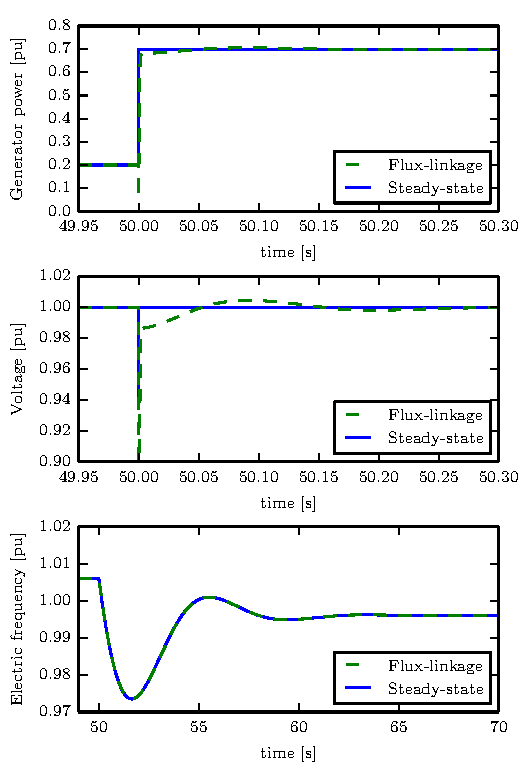
\includegraphics[width=\columnwidth]{figures/fullVsSimplified}
	\caption{Simulation of a step increase of the load from 20\% to 70\% of the rated values. The simulations are done with the models described in Section~\ref{sec:Generator} (steady-state) and models presented in~\cite[Ch.~5.11]{Krause2013} (flux-linkage).}
	\label{fig:fullVsSimplified}
\end{figure}

\subsection{Verification of the Diesel Engine Model}
\label{sec:ICEverification}
A good diesel engine model should be able to predict fuel consumption as well as the engine dynamics in term of speed under transient loads. 
For the prediction of fuel consumption, it is crucial to get a correct fuel consumption curve because the model uses a prescribed cycle efficiency curve rather than actual cycle calculation in the cylinders. 
Such a curve can be obtained by fitting to the given fuel consumption data available for the engine. 

However, the dynamic response of the engine arises from combination of effects from multiple submodels of the system. 
The mean value model used in the simulator alone has about 50 parameters, of which some are arrays. 
Finding proper parameters and tuning the model can be cumbersome process, even if the performance data of the engine is available. 
In order to ease modeling process, one can use a well validated simulation model and normalize the output. 
However, the timescale of the engine dynamics may differ.
Therefore, such a model should be re-tuned to match the dynamics of the engine of interest. 

This can be done by tuning a limited number of parameters which have major influence of the engine response to the load changes. 
In this paper, the gains for the governor controller, the inertia of turbocharger,  the inertia of generator set, and the maximum fuel-air ratio are chosen as tuning parameters. 
The response curve from the load acceptance test of a specific engine was used as reference. 
Then, simulation and optimization are used to curve-fit the simulated response with the reference data. 

The mean value model used in this paper is a generic model for a medium speed four-stroke engine with a reasonable set of parameters. The reference engine is MAN 16V32/44CR which has power rating of 9.6 MW. 
The reference response curve for frequency recovery time and the frequency recovery time vs. step load amplitude plot are used to fit the engine response of the model to the measured value~\cite{MANEnginesandSystems2013}. 
Frequency recovery time is defined as the time interval from the time when the frequency deviates from the steady state band until the time when it again enters the band according to ISO 8528-5. 
Such a band is assumed to be 1\%, and the result of fitting is shown in the Fig.~\ref{fig:MVMResponseTimeCurve}.
\begin{figure}
	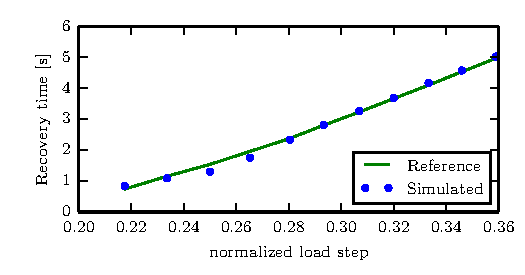
\includegraphics[width=\columnwidth]{figures/MVMResponseTimeCurve.pdf}
	\caption{Dynamic response fitting of diesel engine.}
	\label{fig:MVMResponseTimeCurve}
\end{figure}

\subsection{Verification of the Diesel Engine Constrain Model}
\label{sec:dieselconstraints}
As mentioned in Sec.~\ref{sec:dieselengine}, diesel engine manufacturers constrain the rate of change of the throttle position.
However, a smoke limiter will assure that the throttle position is limited such that complete combustion and maximum torque is achieved.

\begin{figure}
	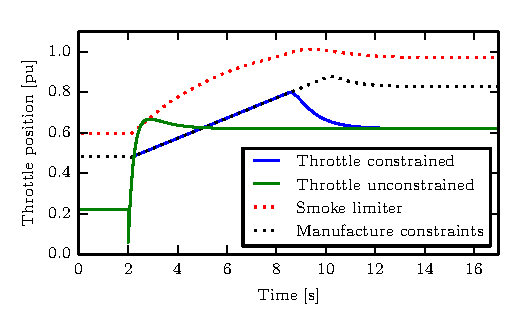
\includegraphics[width=\columnwidth]{figures/withDeadBand}
	\caption{Throttle response of a load step, with and without constraints. The dotted lines represent the manufactures rate constrain and the throttle constraints of the smoke limiter.}
	\label{fig:rateconstrain}
\end{figure}

In Fig.~\ref{fig:rateconstrain}, the earlier presented generator set is subjected to a load step from 20\% active power to 60\%.
The figure shows the responses of the throttle position with and without the smoke limiter and the manufacture constraint activated.
The constraints are also included, showing the smoke limiter level and the manufacture rate constraint.
It is clear that the rate constraint from the manufacture are always lower than the smoke limiter. The smoke limiter can therefore be neglected. 
It should be noted that this result is only valid for this engine.

\section{Case Study}
\label{sec:caseStudy}
Three cases were analyzed, where the objective is to illustrate the simulations that are only possible trough a multi-domain simulator. It is noteworthy that the focus is in the qualitative analysis, but not on quantitative analysis, since the full simulator need to be validates as a whole to be used quantitatively.

A drilling rig is used to illustrate the simulator capabilities, not only for fault scenarios but normal operations as well.
The electrical system is shown in Fig.~\ref{fig:PowerPlantsscheme}.
The rig has three switchboards, which are connected in a ring configuration.
Two generator sets are connected to each switchboard. 
The rated output of the diesel engines are 9.1~MW.
In addition, two thrusters are connected to each switchboard with a rated output of 4.2~MW and a rated thrust of 506~kN. The thrusters position are shown in table \ref{tab:thrusterPosition}.
The rig pontoon length is 84.6~m, with total mass of $27\times10^6$~kg. The dynamic model is assuming low speed, as well as current is considered as a component of the vessel total speed, instead of a force. More detail about the vessel hydrodynamics and physical properties can be found in \cite{MSS2010}.

\begin{table}[!htb]
	\caption{Thruster position on the drilling rig hull}	
	\label{tab:thrusterPosition}
	\begin{center}
	
	\begin{tabularx}{\columnwidth}{ c YYY }
	\hline
		Thruster & Thruster type & X Position [m] & Y position [m] \T\B\\
		\hline			\T
		1 & Azimuth & -35 & -27\\
		2 & Azimuth & -35 & ~27\\
		3 & Azimuth &  ~~0 	& -27\\
		4 & Azimuth &  ~~0 	& ~27\\
		5 & Azimuth &  ~35	& -27\\
		6 & Azimuth &  ~35\B	& ~27  \\ \hline
	\end{tabularx}
	\end{center}
\end{table}


Besides the drilling rig, a hybrid supply vessel was modeled to verify the influence of energy storage devices on the vessel electrical stability. The electrical system is shown in Fig.~\ref{fig:supply}, where one battery pack, one 2.2~MW and one 3.3~MW generators are connected to each power bus. The thruster characteristics are described in Tab.~\ref{tab:thrusterPositionSupply}. The vessel length is 80~m, with total mass of $6.2\times10^6$~kg.


\begin{figure*}[t!]
\centering
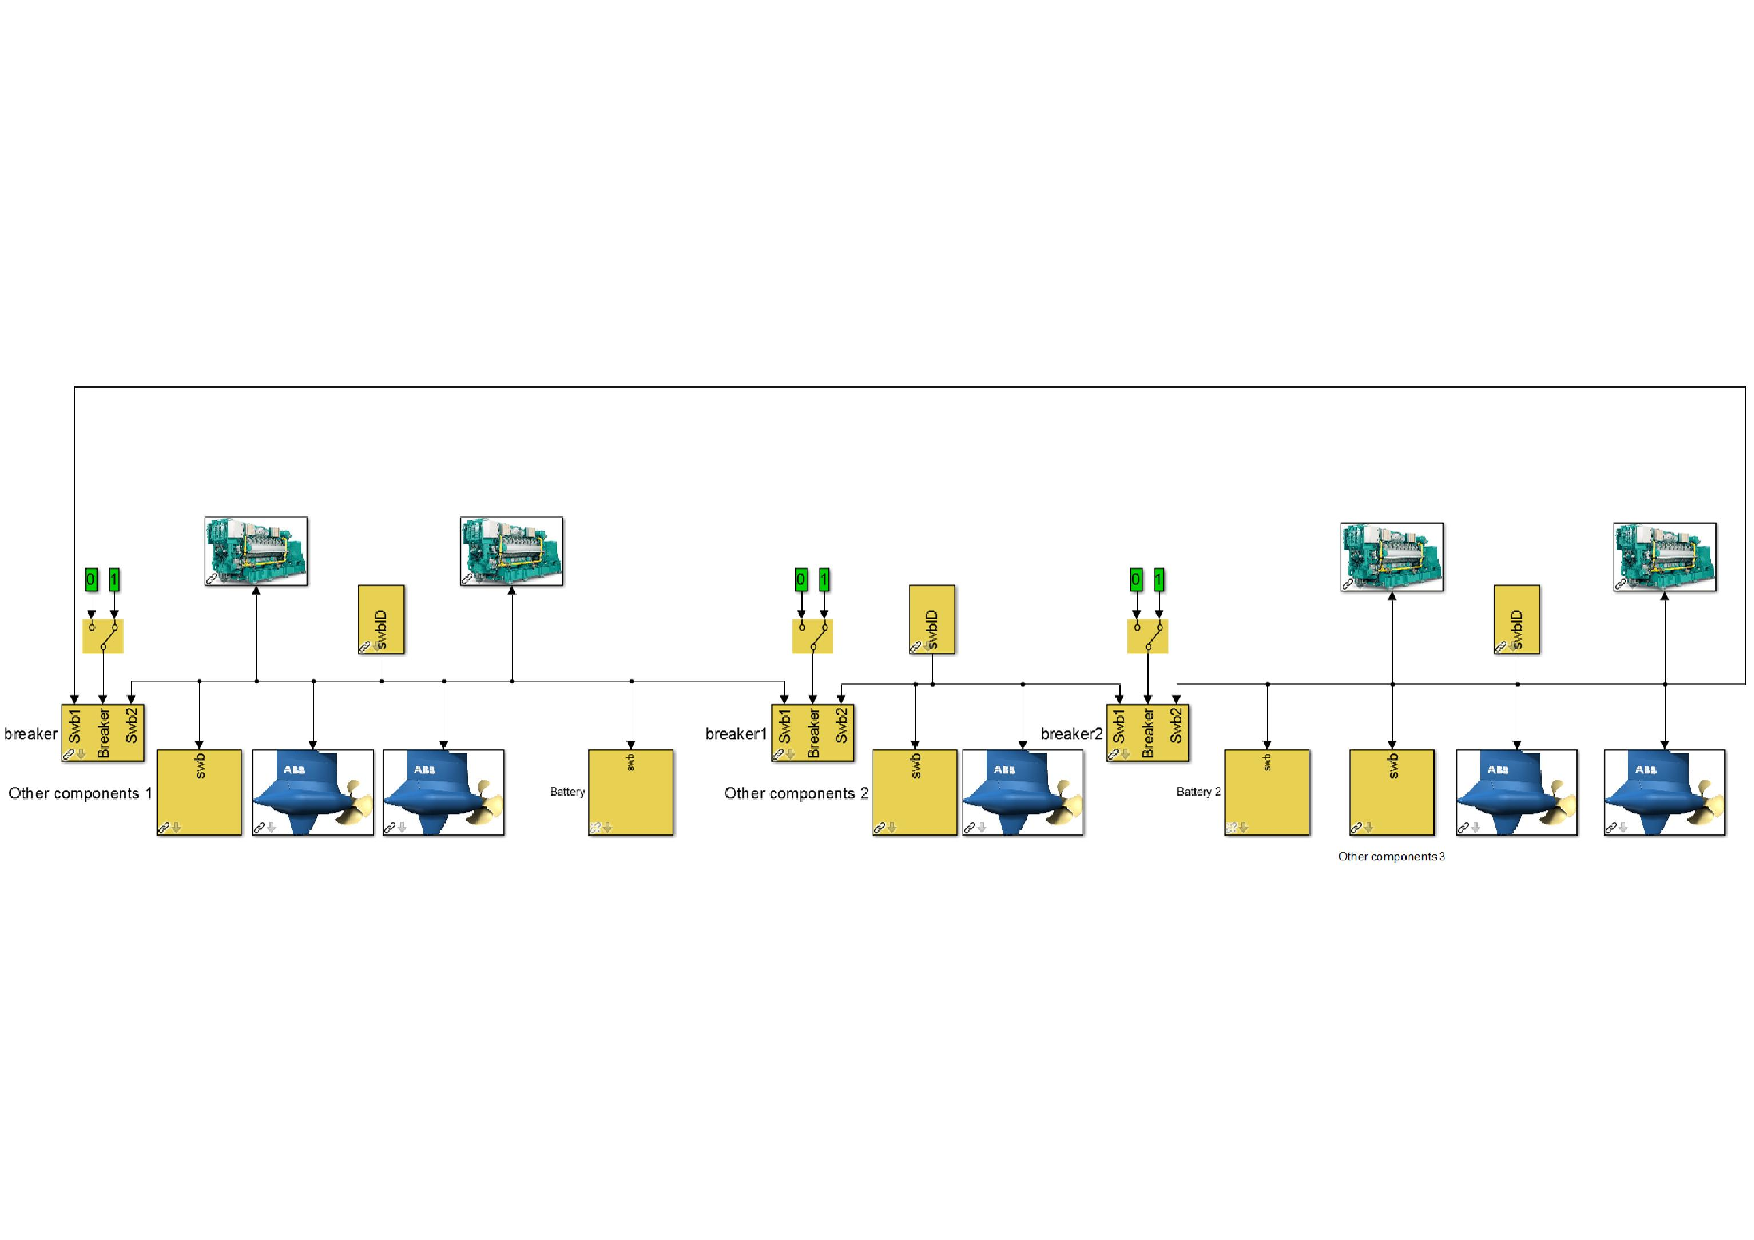
\includegraphics[trim= 0 180 0 180,width=\textwidth,clip]{./figures/supply.pdf}
\caption{Example of power plant view, including the bus tie breakers, thrusters, generator sets, and other loads block. }
\label{fig:supply}
\end{figure*}

\begin{table}[!htb]
	\caption{Thruster position and size on the supply vessel}	
	\label{tab:thrusterPositionSupply}
	\begin{center}
	\begin{tabularx}{\columnwidth}{ rcccY } \hline\T
		Thruster& Type & X Position [m] & Y position [m] & Max Power [MW] \B\\
		\hline			\T
		1 & Azimuth & -30 & -5	& 2.7\\
		2 & Azimuth & -30 &  ~5	& 2.7\\
		3 & Tunnel 	& ~24 &  ~0	& 1.5\\
		4 & Tunnel 	& ~27 &  ~0	& 0.85\\
		5 & Tunnel 	& ~30 &  ~0	& 1.5 \B\\ \hline
	\end{tabularx}
	\end{center}
\end{table}


A summary of all simulation cases environmental condition is shown in table \ref{tab:simSummary}, where the described variables are wave height ($H_s$), wave peak period ($T_P$), wind speed ($V_w$) and current speed ($V_c$). Wind, wave and current direction on all simulation cases are always going from North to South.

\begin{table}[!htb]
	\caption{Environmental condition summary for the simulation cases}	
	\label{tab:simSummary}
	\begin{center}
	\begin{tabularx}{\columnwidth}{ cYYYY } \hline
		Simulation case & $H_S$ [m] & $T_P$ [s] & $V_w$ [m/s] & $V_c$ [m/s] \T\B \\
		\hline \T
		\ref{sec:DPScenario} 	&  5 & 8.5  & 14 & 1 \\
		\ref{sec:busOpening} 	&  2 & 7    & 10 & 1 \\
		\ref{sec:esd} 			&  4 & 7.7  & 12\B & 1 \\ \hline
	\end{tabularx}
	\end{center}
\end{table}

\subsection{DP Operation Scenario}
\label{sec:DPScenario}
The first case study shows a typical DP operation. The goal is to demonstrate the load fluctuation due to environmental forces/DP system and the power generated by the power producers. The position and heading setpoints are fixed at the origin. The buses are connected in a ring configuration, with all bus tie breakers closed. 
Irregular waves are present in this case, with significant wave height of $5~m$, peak frequency of $7~s$ and JONSWAP wave spectrum \cite{Myrhaug2000}. 
The wind speed is set to the expected value for this sea state, given by the JONSWAP wave spectrum.


\begin{figure}
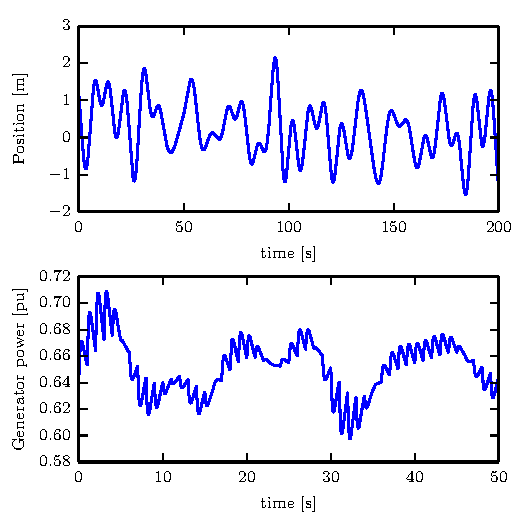
\includegraphics[width=\columnwidth]{figures/dpIrregular}
\caption{Surge position and electric bus frequency of the analyzed drilling for the simulation presented in Sec.~\ref{sec:DPScenario}.}
\label{fig:DPIrregular}
\end{figure}

Fig.~\ref{fig:DPIrregular} shows the vessel surge position and electric bus frequency for the simulated case. Notice that the simulator is able to capture different time scales and time constant in the vessel positioning and the generator power.
A power variation of same time scale as the wave frequency is clearly visible.
In addition, the change of thruster set-point gives ripples at 1~Hz.


\subsection{Bus Opening Scenario}
\label{sec:busOpening}
During a DP operation, it is possible that one bus is isolated from the remaining grid due to a pre-fault detection, reverse power flow, etc. In this case the interaction between the electrical system and the DP system is exemplified. Even though the maximum generated capability and thruster forces are unaltered, there is a instantaneous power surge in the buses due to the reconfiguration.

In the simulation, the vessel is in DP~operation and heading north, with closed bustie and five generator sets running (two connected to each of the first two switchboard and one to the third switchboard).
Switchboard~3 is separated from the other two switchboards, by opening the breakers connected to Switchboard~3 at $t = 200$ s.
The power consumption is constrained by the fast load reduction, due to the increased load.
The waves have significant wave height of 2~m, peak frequency of 7~s and JONSWAP wave spectrum \cite{Myrhaug2000}. The wind is simulated using the NORSOK wind spectrum \cite{Sorensen2013}, with $U~=~10$~m/s.

\begin{figure}
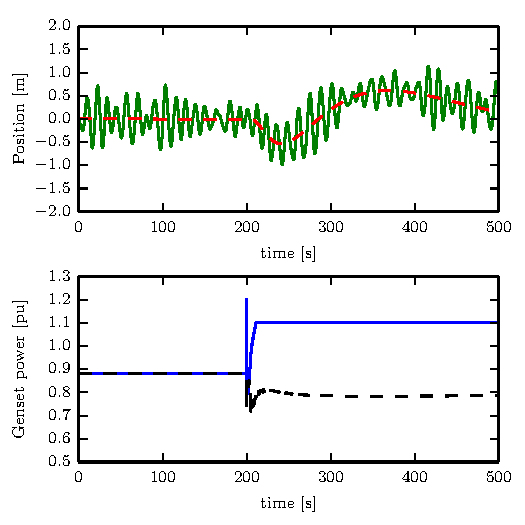
\includegraphics[width=\columnwidth,clip]{figures/busIsolation}
\caption{Vessel positioning and power consumption for both the isolated and main power grid for the simulation case presented in Sec.~\ref{sec:busOpening}. In the position plot, the green solid line is the position deviation from the set-point. The red dashed line is the position deviation without the wave motion. In the lower plot, the blue solid line and the black dashed line are the generator power of the generators at the isolated power grid (swb~3) and main power grid (swb~1 and~2), respectively.}
\label{fig:busPosition}
\end{figure}

Fig.~\ref{fig:busPosition} shows the power bus reconfiguration effect on the dynamical positioning system. It is noticeable that when the power plant is reconfigured, the DP system positioning is influenced due to load reduction.
This scenario can only be simulated with an integrated simulator, since the interdependency in the positioning system and electrical system is the factor leading to the positioning transient.

Both the vessel positioning and the filtered position (estimated by the state estimator) are presented in Fig.~\ref{fig:busPosition}, since the wave frequency motion makes it harder to observe the mentioned effect.


%\subsection{Faulty Scenario}
%\label{sec:fault}
%In the simulation, the vessel is in DP~operation and heading north, with closed bustie and five generator sets running (two connected to each of the first two switchboard and one to the righter most switchboard).
%Switchboard~1 is separated from the other two switchboards, by opening the breakers connected to Switchboard~1 after 50~seconds.
%The power consumption is constrained by the fast load reduction, due to the increased load on Switchboard~2 and~3.
%50~seconds later, the last generator connected to Switchboard~3 is disconnected.
%A thruster connected to Switchboard~3 is disconnected 2 seconds after the disconnection of the generator.
%To avoid underfrequency the fast load reduction reduces the thrust.
%The PMS uses the power available signal to avoid overload of the generators after the fast load reduction has increased its constraints.
%The thrust allocation is then able to redistribute the thrust between the buses, since the power available signal is directed to the thrust allocation.
%
%As is seen in Fig.~\ref{fig:caseplot} we are able to simulate this fault scenario.
%We are also able to simulate how the safety systems respond and how this influence the position accuracy and power plant.
%Also note that the power consumption of the thrusters are fluctuating before the faults occur.
%This is due to the wave induced motions of the vessel, which gives fluctuating advance velocity of the propeller.
%Switchboard~1 is also increasing its thruster loads after the loss of a generator and thruster at Switchboard~3.
%This is done since the thruster loads is at the power available limit for Switchboard~2 and~3.
%Some position deviation from the setpoint occurs after the fault; this is due to the reconfiguration and loss of power after the fault.
%
%\begin{figure}
%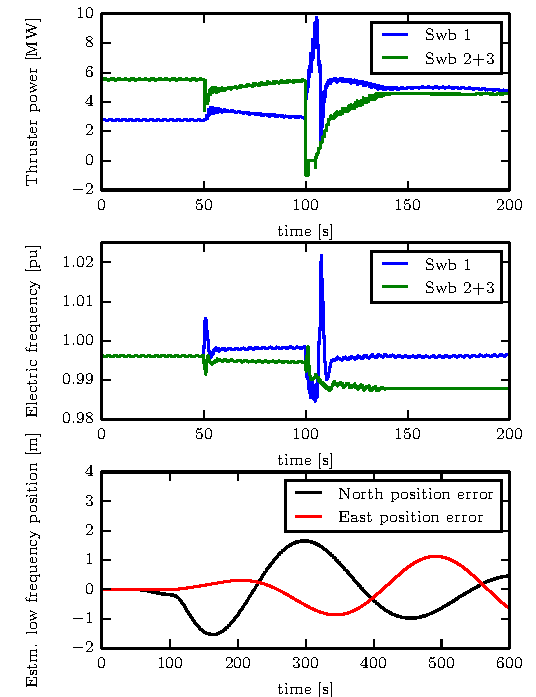
\includegraphics{figures/omae}
%\caption{Power consumption of thrusters, electric frequency, and position deviation from DP~set-point for simulation presented in section ``Case study''}
%\label{fig:caseplot}
%\end{figure}

\subsection{Energy storage devices}
\label{sec:esd}
The last case analyzed demonstrates how the addition of an an energy storage device will increase overall safety, mostly due to the fact that the extra power injection in the buss will limit the frequency drop by the generator. The system presented here uses the supply vessel presented in section \ref{sec:caseStudy}. All four generators and five thrusters are initially connected. An \ac{ESD} is connected to the power system. The wind is simulated using the NORSOK wind spectrum as well as JONSWAP wave spectrum. After 10~seconds, one of the generators is abruptly disconnected  from the power grid, generating a power surge for the remaining three generators. The \ac{ESD} is controlled in frequency droop mode, but it will be connected only when the frequency drops below 98.5\%.


The results from this scenario are shown in Fig.~\ref{fig:esdCase}. The vessel position is virtually the same for both simulation cases, the main difference is that the frequency drop is much smaller in the case with \ac{ESD}. It is know, that protection systems like load reduction and shedding will be activated when the frequency drops below 2\% to 3\%, possibly deactivating large power consumers, such as thrusters, drilling system, etc. If the frequency drops even further, it could lead to partial or even total blackout.

From the maintenance point of view, with smoother generator load variation, the wear and tear will be reduced, improving the generator working conditions and reducing maintenance costs.

This simulation shows that the simulator is able to verify the vessel and \ac{ESD} dynamical behavior during a fault, in which the frequency drop is the main concern. The \ac{ESD} is able to bound the frequency drop to a safe margin, potentially preventing a larger scale fault.

Other operation strategies may be implemented for the \ac{ESD}, such as peak shaving, on-off operations, etc, but that is beyond the scope of this paper.

\begin{figure} % width 252pt
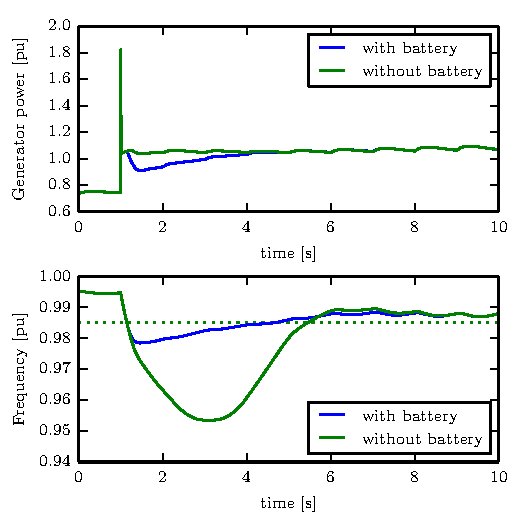
\includegraphics[width=\columnwidth]{figures/esdCase}
\caption{Generator power and bus line frequency for the simulation presented in section \ref{sec:esd}}
\label{fig:esdCase}
\end{figure}


%\subsection{Further Work}
%Such a simulator as presented can always be extended to higher fidelity and include new models and control strategies.
%Some models which may be added are low level protection system, such as undervoltage/-frequency relay.
%The simulator is not able to connect two buses during a simulation since the switchboards may not be synchronized.
%To be able to do so a bus synchronizer is needed, which will adjust the no load frequency of the generator sets.


\section*{Conclusion}
\label{sec:conclusion}
In this article, a simulator for marine vessels electric propulsion is presented.
The main contribution is the presentation and verification of the needed models for the integration of power plant simulation and vessel motion simulation as well as the demonstration of the integrated simulator, enabling the qualitative analysis of cases that would require several decoupled simulators.
The system simulator includes detailed models of the vessel, propeller, thruster drives, generator sets, and controllers, in addition to interaction effects between the components.
The simulator is module based and models of different fidelity can be chosen.
Due to the modularity, the simulator can be reconfigured to many different vessels with electric propulsion, and different operations can be simulated.
Simulink is used to implement the simulator and the simulator can run on NI cRIO in real-time.
The case studies presented in the article show some of the capabilities of the simulator. More detailed simulations of, e.g.,  fault scenarios contribute to increased knowledge about the behavior of the electrical system, control systems, and safety functions, which may lead to more reliable vessels and safer operations in the future. 




\bibliography{main} 
\bibliographystyle{IEEEtran}
\todos
\end{document}


